\documentclass[a4paper]{article}

% Basic packages
\usepackage{fontspec}
\XeTeXlinebreaklocale "zh"    % 启用中文断行（XeTeX 内建，无需 xeCJK）
\XeTeXlinebreakskip = 0pt plus 1pt
\setmainfont{Songti SC}
\setsansfont{Heiti SC}
\setmonofont{Menlo}
\usepackage{amsmath, amssymb}
\usepackage{graphicx}
\usepackage[margin=2.5cm]{geometry}
\usepackage[most]{tcolorbox}
\usepackage{etoolbox}
\usepackage{listings}
\usepackage{hyperref}
\usepackage{booktabs}
\usepackage{subcaption}
\usepackage{float}

% Chinese font setup (macOS system fonts, no ctex needed)
\setmainfont{Songti SC}
\setsansfont{Heiti SC}
\setmonofont{Menlo}
\newcommand{\song}{\fontspec{Songti SC}}
\newcommand{\hei}{\fontspec{Heiti SC}}
\newcommand{\kai}{\fontspec{KaiTi}}
\newcommand{\fangsong}{\fontspec{FangSong}}

% ===== Highlight boxes =====
\newtcolorbox{knowledgebox}[1]{
    enhanced, colback=blue!5!white, colframe=blue!75!black, colbacktitle=blue!75!black,
    coltitle=white, fonttitle=\bfseries, title=#1, attach boxed title to top left={yshift=-2mm, xshift=2mm},
    boxrule=1pt, sharp corners
}

\newtcolorbox{importantbox}[1]{
    enhanced, colback=yellow!10!white, colframe=yellow!80!black, colbacktitle=yellow!80!black,
    coltitle=black, fonttitle=\bfseries, title=#1, sharp corners
}

\newtcolorbox{warningbox}[1]{
    enhanced, colback=red!5!white, colframe=red!75!black, colbacktitle=red!75!black,
    coltitle=white, fonttitle=\bfseries, title=#1, sharp corners
}

\newtcolorbox{practicebox}[1]{
    enhanced, colback=green!5!white, colframe=green!60!black, colbacktitle=green!60!black,
    coltitle=white, fonttitle=\bfseries, title=#1, sharp corners
}

% ===== Code listings =====
\lstset{
    basicstyle=\ttfamily\small,
    keywordstyle=\color{blue},
    stringstyle=\color{red!60!black},
    commentstyle=\color{green!60!black},
    breaklines=true,
    frame=single,
    numbers=left,
    numberstyle=\tiny\color{gray},
    captionpos=b,
    extendedchars=false
}

% ===== Front-page metadata =====
\newcommand{\notetitle}{CS336 Lecture 5：GPU 与 CUDA 性能剖析}
\newcommand{\notesubtitle}{Stanford CS336: Language Modeling from Scratch (Spring 2025)}
\newcommand{\noteauthors}{讲师：Percy Liang, Tatsu Hashimoto \quad 笔记：ZCode}
\newcommand{\notedate}{2026-07-14}
\newcommand{\videochannel}{Stanford CS336}
\newcommand{\videopublishdate}{2025 Spring}
\newcommand{\videoduration}{74 分钟}
\newcommand{\videourl}{https://www.youtube.com/watch?v=nUuoGrJZaj8}
\newcommand{\videocoverpath}{cover.jpg}

\begin{document}

% ===== Title page =====
\begin{titlepage}
\centering
{\Large 课程笔记\par}
\vspace{1.2cm}
{\huge\bfseries \notetitle\par}
\vspace{0.3cm}
{\large \notesubtitle\par}
\vspace{0.5cm}
{\large \noteauthors\par}
\vspace{0.3cm}
{\large \notedate\par}
\vspace{1.0cm}

\includegraphics[width=0.82\textwidth,height=0.40\textheight,keepaspectratio]{\videocoverpath}\par

\vfill
\begin{tcolorbox}[width=0.9\textwidth, colback=black!2!white, colframe=black!60, sharp corners]
\textbf{视频作者/频道}：\videochannel\par
\textbf{发布日期}：\videopublishdate\par
\textbf{视频时长}：\videoduration\par
\textbf{视频链接}：\href{\videourl}{\nolinkurl{\videourl}}
\end{tcolorbox}
\end{titlepage}

\tableofcontents
\newpage

%% --- 正文内容开始 ---

\section{引言：为什么要理解 GPU 与 CUDA}

\subsection{让 CUDA 和 GPU 不再神秘}

本讲是 CS336 课程硬件系列的第二讲，聚焦于 GPU 这一当下深度学习最主要的加速器。讲师开门见山地给出了本讲的目标：\textbf{让 CUDA 和 GPU 不再神秘（Make CUDA and GPUs less magic）}。许多同学都用过 PyTorch 调 \texttt{nn.Linear}、调用过 attention，但当你在终端里看到一段 CUDA kernel 的报错，或是看到矩阵乘法在不同尺寸下吞吐量剧烈起伏时，往往会觉得"GPU 像个黑箱"。本讲就是要拆开这个黑箱。

\begin{figure}[H]
\centering
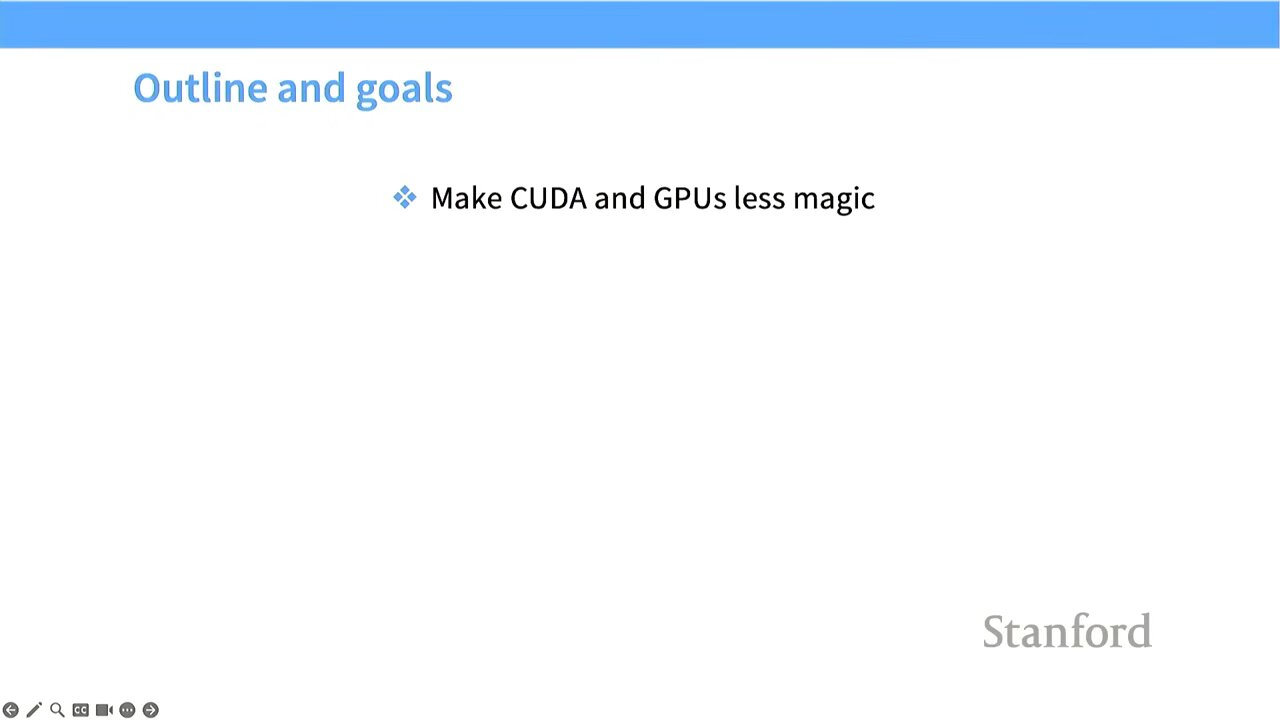
\includegraphics[width=\textwidth]{figures/fig_01_outline.jpg}
\caption{课程大纲：让 CUDA 和 GPU 不再神秘\protect\footnotemark}
\end{figure}
\footnotetext{视频画面时间区间：00:00:30--00:00:45。}

讲师把整讲内容划分为三大块。第一部分是\textbf{硬件与执行模型}：把 GPU 当作一个独立的加速器，深入理解它的内部结构（SM、SP、张量核、内存层次）和它如何执行一段 CUDA 程序（block、warp、thread）。同时会非常简略地对比 TPU，因为 TPU 在很多概念上和 GPU 高度相似，理解了 GPU 也就理解了 TPU 的大部分思路。

第二部分是\textbf{性能分析}：在理解了硬件之后，回答"什么让 GPU 在某些负载上快、在另一些负载上慢"。这一部分会引入 roofline 模型、算术强度、内存瓶颈与计算瓶颈的判定，并通过一个贯穿全讲的"矩阵乘之谜"把所有概念串起来。

第三部分是\textbf{实战 Flash Attention}：把前面学到的所有技巧（低精度、算子融合、重计算、内存合并、分块）综合起来，手把手走一遍 Flash Attention，看它如何把 attention 的 HBM 访问降到亚平方量级。

\begin{knowledgebox}{本讲的三大目标}
\begin{enumerate}
\item 理解 GPU 的硬件与执行模型（SM、warp、内存层次）。
\item 掌握判断 GPU 负载性能的方法（roofline、算术强度）。
\item 把五个核心优化技巧运用到 Flash Attention 上。
\end{enumerate}
\end{knowledgebox}

\subsection{为什么硬件如此重要：算力缩放定律}

在正式进入 GPU 之前，讲师先用一张缩放定律的图设定背景。在 NLP 课程里大家都见过 pre-training scaling chart：横轴是算力（FLOPs），纵轴是模型性能，基本是单调上升的。这背后的逻辑很直接——\textbf{算力越多，能处理的数据越多，能训练的模型越大，性能就越好}。深度学习算法当然重要，但真正驱动过去十年性能飞跃的，是更快硬件、更高利用率、更强的并行化。

\begin{figure}[H]
\centering
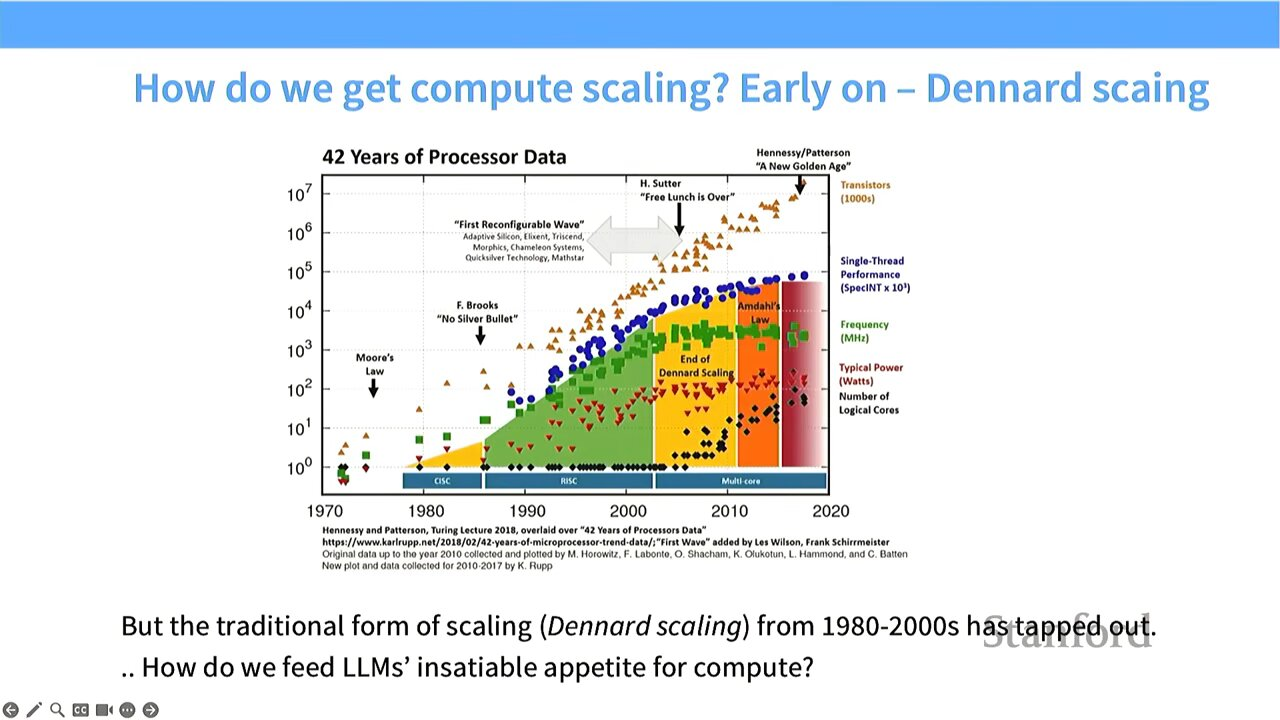
\includegraphics[width=\textwidth]{figures/fig_02_dennard.jpg}
\caption{Dennard 缩放在 2000 年代后失效，单线程性能停滞\protect\footnotemark}
\end{figure}
\footnotetext{视频画面时间区间：00:04:45--00:05:00。}

但算力从哪里来？在半导体缩放的早期，CPU 性能的提升依赖两条腿：摩尔定律（晶体管密度翻倍）和 \textbf{Dennard 缩放}（晶体管越小，可以跑得越快、功耗越低）。这两者叠加，让单线程性能在 1980 到 2000 年代持续飙升。Hennessy 与 Patterson 的经典图表显示，大约在 2000 年代中后期，单线程性能（图中蓝点）开始明显放缓——晶体管密度还在涨，但单线程吞吐不再受益。这就是著名的\textbf{"功耗墙"}与 Dennard 缩放的终结。

\begin{warningbox}{Dennard 缩放的终结意味着什么}
单线程性能停滞 = "绝对速度"不能再无脑涨。要继续提升算力，唯一出路是\textbf{并行缩放}：用大量低频核心一起干活，而非追求单核高频。这正是 GPU 的设计哲学。
\end{warningbox}

\begin{figure}[H]
\centering
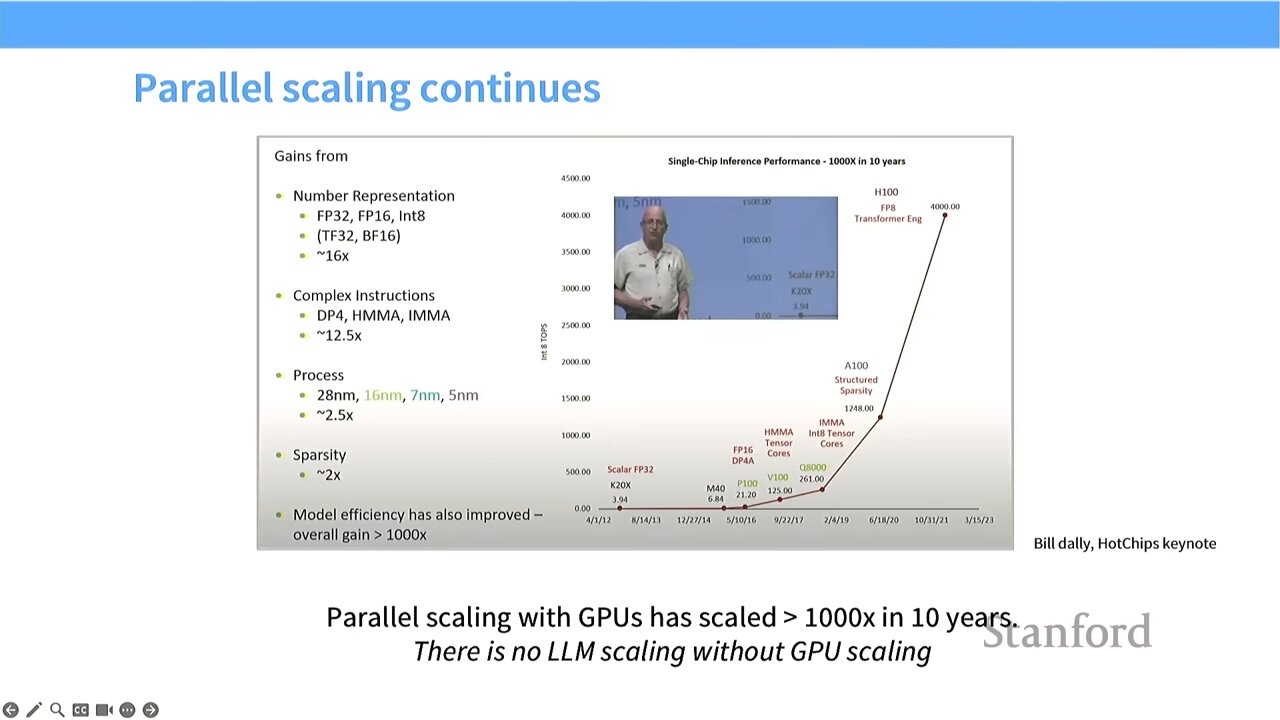
\includegraphics[width=\textwidth]{figures/fig_03_parallel_scaling.jpg}
\caption{Bill Dally 的主题演讲：NVIDIA GPU 整数算力的超级指数曲线\protect\footnotemark}
\end{figure}
\footnotetext{视频画面时间区间：00:05:45--00:06:00。}

讲师展示了他最喜欢的一张图——NVIDIA 首席科学家 Bill Dally 的 keynote 曲线：从早期的 K20 一路到 H100，GPU 每秒整数运算次数走出了一条\textbf{超级指数（super-exponential）}的增长曲线。这正是并行缩放的红利。要真正榨干这条曲线来训练语言模型，就必须深入理解 GPU 的工作方式。

\section{CPU vs GPU：延迟与吞吐的设计哲学}

在进入 GPU 内部细节之前，讲师先用一个抽象对比建立直觉。\textbf{CPU 优化延迟（latency），GPU 优化吞吐（throughput）}，这是两者最根本的设计哲学差异。

\begin{figure}[H]
\centering
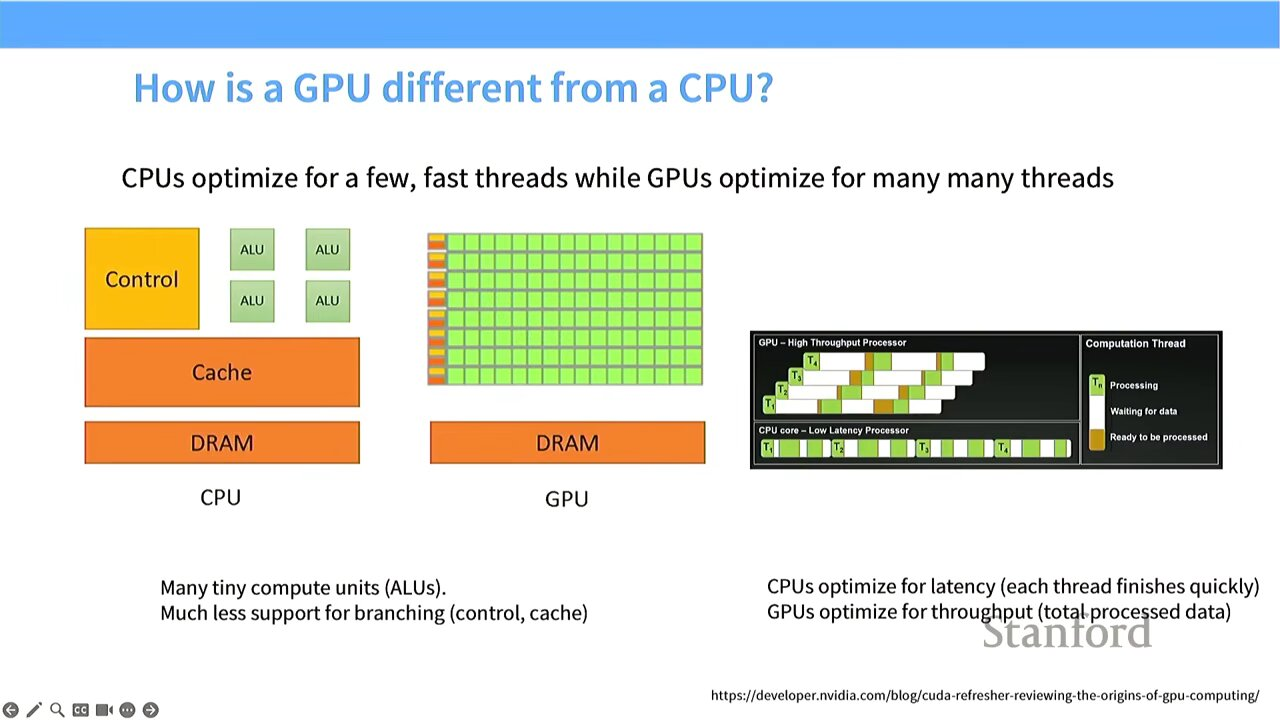
\includegraphics[width=\textwidth]{figures/fig_05_cpu_vs_gpu.jpg}
\caption{CPU 为延迟优化、GPU 为吞吐优化的不同设计取向\protect\footnotemark}
\end{figure}
\footnotetext{视频画面时间区间：00:08:15--00:08:30。}

CPU 的执行模型是：一段程序、一个线程、一步一步往前走。为了支持这种模型并尽量把单线程跑快，CPU 把大量芯片面积花在\textbf{大型控制单元、分支预测、乱序执行、深缓存}上。它的目标是让任务 $T_1$ 尽快完成。现在的 CPU 当然也有多核，但和 GPU 比起来，核数几乎可以忽略不计。

GPU 则反其道而行：芯片上塞满了大量的计算单元（ALU），每个控制单元只占很小的面积，用一点控制逻辑去编排海量并行计算单元。单个任务的延迟可能比 CPU 还高，但当有成千上万个任务 $T_1 \dots T_n$ 一起涌入时，GPU 可以让大量线程快速睡眠与唤醒，最终\textbf{在总体上}比 CPU 更快地把所有任务做完。

\begin{importantbox}{延迟 vs 吞吐的直觉}
假设你要处理 4 个任务。CPU 像一辆跑车，$T_1$ 立刻完成、$T_2$ 紧随其后，单看每个都快，但总量有限。GPU 像一支 256 辆公交组成的车队，单辆车又慢又笨重，但一次能把 256 个任务同时运走。当任务量足够大，车队完胜。
\end{importantbox}

这种"用并行掩盖延迟"的思路是后面所有内容的基石：\textbf{只要你有足够多的可并行工作，GPU 就能让它的计算单元一直忙碌}；反之，如果工作太少或并行度不够，GPU 的吞吐优势就发挥不出来。

\section{GPU 的硬件解剖}

\subsection{SM、SP 与张量核}

理解了设计哲学，现在拆开 GPU 看内部结构。NVIDIA GPU 的核心计算单元是 \textbf{SM（Streaming Multiprocessor，流式多处理器）}。每个 SM 内部又有大量更细粒度的 \textbf{SP（Streaming Processor，流式处理器）}，可以理解为最基础的标量计算单元。此外，每个 SM 还内建了专门用于矩阵乘的\textbf{张量核（Tensor Core）}。

\begin{figure}[H]
\centering
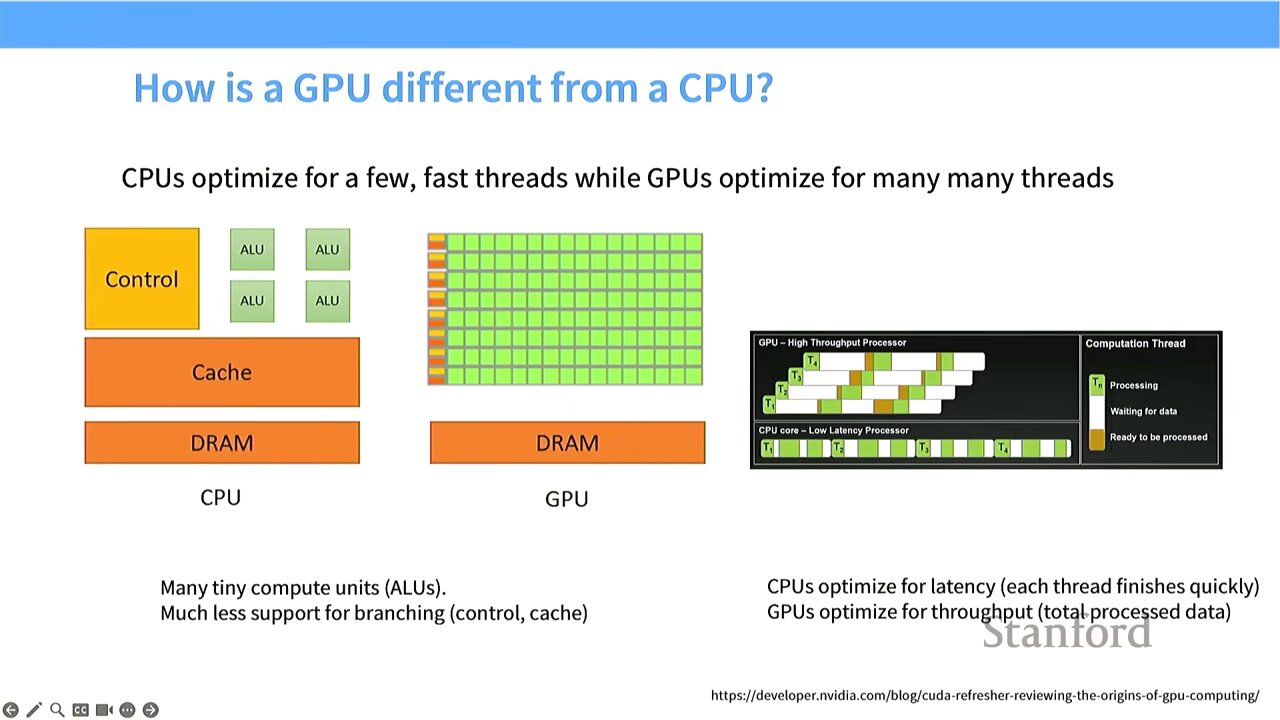
\includegraphics[width=\textwidth]{figures/fig_04_gpu_anatomy_sm.jpg}
\caption{GPU 解剖：SM 内含大量 SP 与专用矩阵乘单元（张量核）\protect\footnotemark}
\end{figure}
\footnotetext{视频画面时间区间：00:06:30--00:06:45。}

讲师以 A100（上一代旗舰 GPU）为例给出关键数字。整个 GPU 的峰值算力可以粗略地表示为各 SM 算力之和：

\[
\text{peak FLOPS}_{\text{GPU}} = N_{\text{SM}} \times \text{FLOPS}_{\text{per SM}}
\]

\begin{center}
\begin{tabular}{ll}
\toprule
\textbf{指标} & \textbf{A100} \\
\midrule
SM 数量 & 128 \\
每 SM 内含 & 大量 SP + 专用矩阵乘单元（张量核） \\
类比 CPU & 128 个 SM 远多于任何 CPU 的核数 \\
\bottomrule
\end{tabular}
\end{center}

128 个 SM 是什么概念？这比绝大多数 CPU 的核心数高出一到两个数量级。而且每个 SM 内部又有非常多的 SP 和专用的矩阵乘单元。讲师用一个卡通图解释：你可以把 GPU 的每一"行"想象成一个 SM，它有自己的控制单元；每一行里的绿色小方块就是一个 SP 一类的处理单元。整个 GPU 的计算模型，就是让这 128 个 SM 各自独立、又协调地处理海量数据。

\begin{knowledgebox}{为什么 GPU 这么适合深度学习}
GPU 之所以在深度学习时代一统天下，根本原因是它\textbf{极易横向扩展}：想要更多算力，就堆更多 SM，不必像 CPU 那样追求更高的时钟频率（会带来严重的散热与功耗问题）。深度学习的核心运算——矩阵乘——天然高度并行，正好契合 GPU "海量简单核心"的设计。
\end{knowledgebox}

\subsection{内存层次：物理邻近决定访问速度}

计算只是 GPU 性能的一半，\textbf{另一半、甚至更重要的一半，是内存}。讲师强调，要理解 GPU 的内存性能，必须理解芯片的\textbf{物理布局}：当工作在如此高的频率下，内存与计算单元的物理距离直接决定了访问延迟。越靠近计算单元的存储越快但也越小、越贵；越远的越大但越慢。

\begin{figure}[H]
\centering
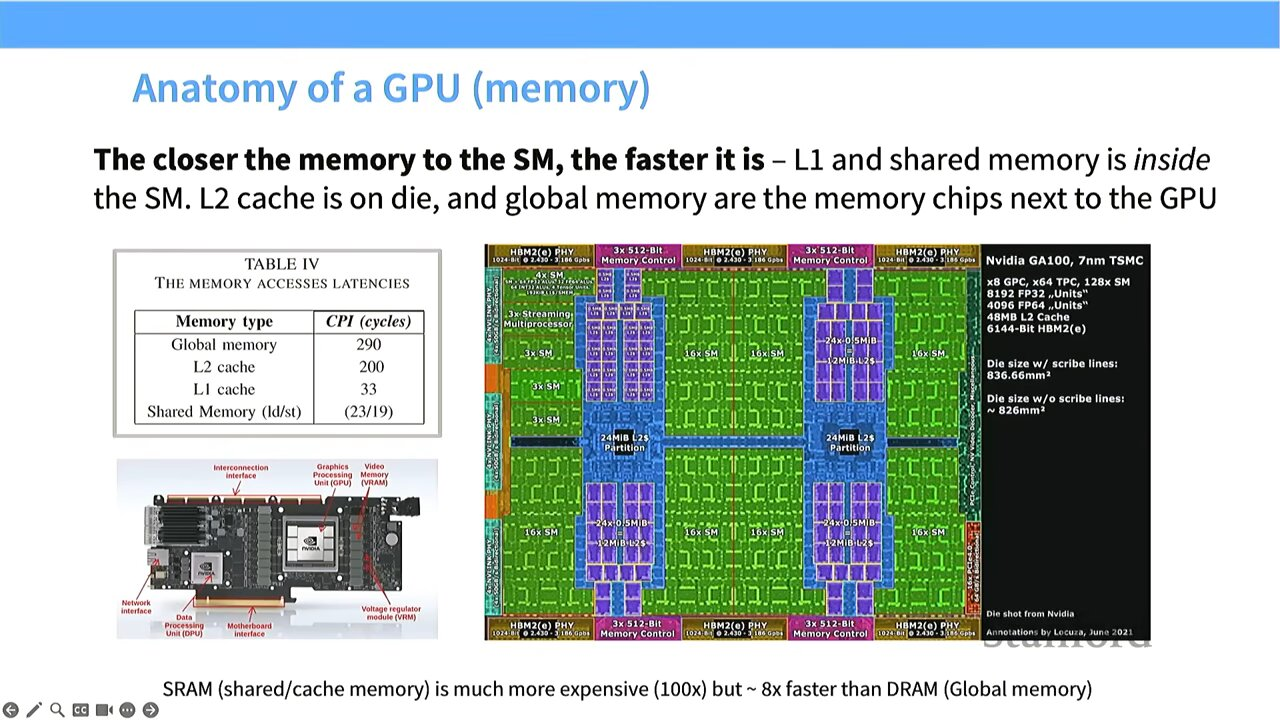
\includegraphics[width=\textwidth]{figures/fig_06_gpu_anatomy_mem.jpg}
\caption{GA100 芯片布局：L1/共享内存在 SM 内，L2 与全局/HBM 在外\protect\footnotemark}
\end{figure}
\footnotetext{视频画面时间区间：00:10:45--00:11:00。}

从这张 GA100 的 die shot 可以清晰看到内存的层次结构。归纳起来，GPU 的内存层次大致如下：

\begin{center}
\begin{tabular}{llll}
\toprule
\textbf{层级} & \textbf{位置} & \textbf{量级（延迟）} & \textbf{说明} \\
\midrule
寄存器（registers） & SM 内 & 最快（约 1 周期） & 每线程私有，容量极小 \\
L1 / 共享内存（shared） & SM 内 & 约 20 周期 & 同一 block 的线程可共享 \\
L2 cache & 芯片上、SM 外 & 约 200--300 周期 & 所有 SM 共享 \\
全局内存 / DRAM / HBM & 芯片外 & 最慢（数百周期） & 容量最大，但延迟最高 \\
\bottomrule
\end{tabular}
\end{center}

\begin{importantbox}{内存是性能的关键}
讲师明确指出，在今天以及可见的未来，\textbf{内存（带宽与延迟）比计算本身更重要}，它在决定 GPU 程序性能上的权重会持续上升。后面所有的优化技巧，本质上都在解决"如何减少对慢速全局内存的访问"。
\end{importantbox}

\section{GPU 的执行模型：block、warp 与 thread}

理解了硬件，接下来看一段 CUDA 程序在 GPU 上是怎么被执行的。这是连接"硬件"和"软件优化"的桥梁。CUDA 的编程模型采用 \textbf{grid $\to$ block $\to$ warp $\to$ thread} 的层次结构。

\begin{figure}[H]
\centering
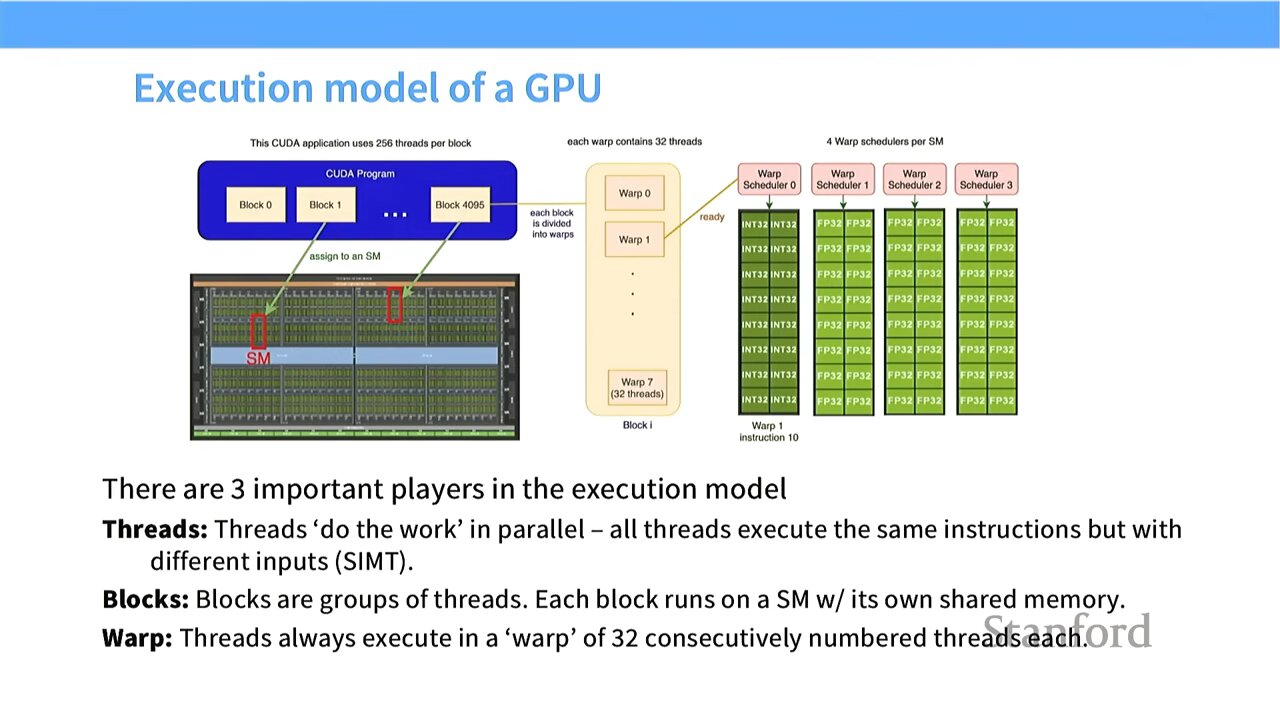
\includegraphics[width=\textwidth]{figures/fig_07_execution_model.jpg}
\caption{GPU 执行模型：block 被分配到 SM，block 内按 warp（32 线程）调度\protect\footnotemark}
\end{figure}
\footnotetext{视频画面时间区间：00:13:45--00:14:00。}

在 CUDA 编程模型里，程序员写的是一个 \textbf{kernel}，它会在一个 \textbf{grid}（网格）上被并发执行。一个 grid 由若干 \textbf{block}（线程块）组成，每个 block 会被分配到某个 SM 上运行。block 内部又被硬件划分为若干 \textbf{warp}，每个 warp 由固定数量的线程组成。在 NVIDIA GPU 上：

\begin{warningbox}{warp 的关键事实}
一个 \textbf{warp 恒为 32 个线程}。这 32 个线程在同一个时钟周期内执行\textbf{完全相同的指令}（这就是 SIMT，Single Instruction, Multiple Threads）。warp 是 GPU 调度和执行的基本单位——不存在"半个 warp"在跑。
\end{warningbox}

形式化地说，一个 block 内的线程数 $T_{\text{block}}$ 与 warp 数 $N_{\text{warp}}$ 的关系为：

\[
N_{\text{warp}} = \left\lceil \frac{T_{\text{block}}}{32} \right\rceil
\]

例如 block 含 64 个线程，就是 2 个 warp；含 100 个线程，向上取整得 4 个 warp（最后一个 warp 有 28 个线程空转）。这也是为什么 block 大小通常取 32 的倍数。

这就是 SIMT 执行模型的核心：硬件以 warp（32 线程）为粒度调度，同一个 warp 内的所有线程锁步（lockstep）地执行同一条指令，只是各自操作不同的数据。这种设计让控制逻辑极简——只需要一套指令译码和派发，就能驱动 32 个计算单元。

\subsection{逻辑内存模型：线程、block 与 SM 的可见性}

执行模型与内存模型是配套的。CUDA 暴露给程序员的逻辑内存模型，严格对应到硬件层次：

\begin{figure}[H]
\centering
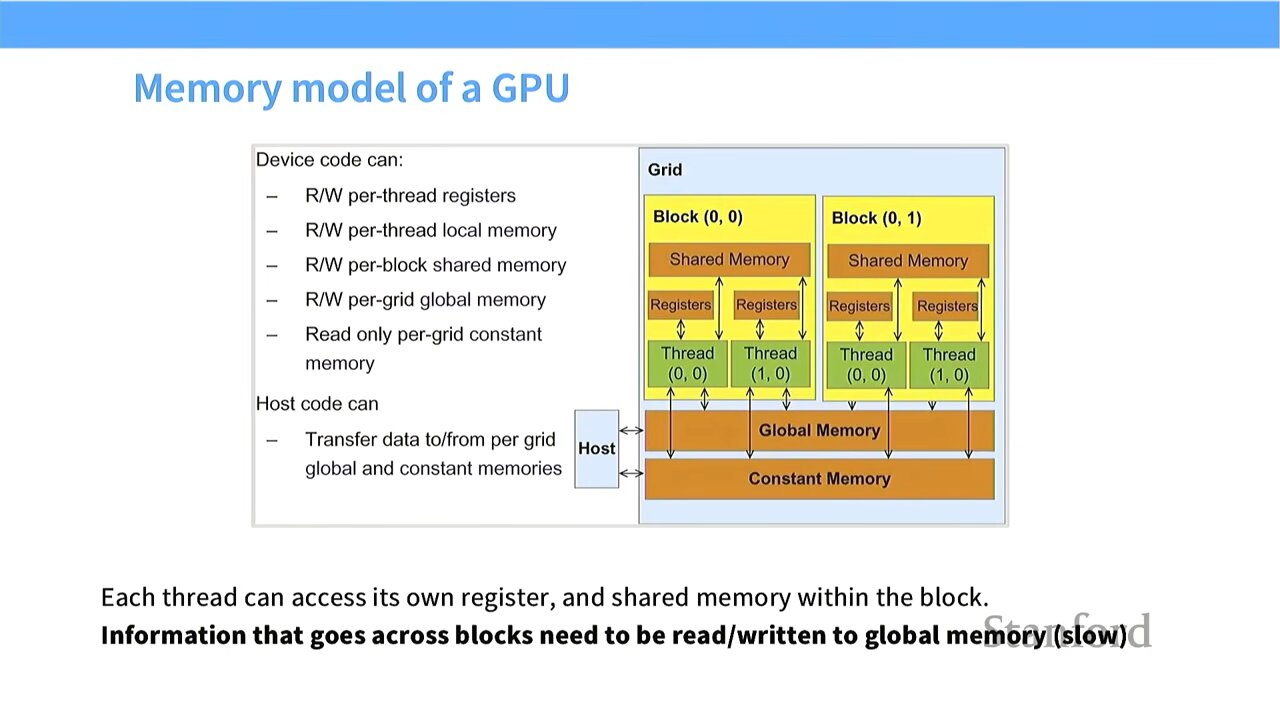
\includegraphics[width=\textwidth]{figures/fig_08_memory_model.jpg}
\caption{CUDA 逻辑内存模型：寄存器、共享、全局、常量内存的可见性\protect\footnotemark}
\end{figure}
\footnotetext{视频画面时间区间：00:15:15--00:15:30。}

\begin{itemize}
\item \textbf{寄存器}：每个线程私有，最快。
\item \textbf{共享内存（shared memory）}：同一个 block 内的所有线程可见，由该 block 所在的 SM 提供，速度接近寄存器。这是程序员显式管理的高速缓存。
\item \textbf{全局内存（global memory）}：所有线程（所有 block、所有 SM）可见，但位于芯片外的 HBM，速度最慢。这就是大家常说的"显存"。
\item \textbf{常量内存 / 纹理内存}：带有特殊缓存机制的全局内存，用于只读场景。
\end{itemize}

\begin{practicebox}{编程心法：把热数据搬到共享内存}
高性能 CUDA kernel 的核心套路就是：\textbf{把反复使用的数据一次性从慢速全局内存搬到快速共享内存，之后所有重用都在共享内存里完成}。这一思路会在后面"分块（tiling）"一节正式登场，并贯穿 Flash Attention。
\end{practicebox}

\section{TPU：另一种加速器，相同的内核思想}

讲师非常简短地提了一下 TPU，强调\textbf{TPU 在概念上和 GPU 高度相似}。理解了 GPU，就理解了 TPU 的大部分。一个 TPU 的核心叫 \textbf{tensor core}（注意这里的 tensor core 概念层级相当于 GPU 的 SM，而不是 GPU 里的 tensor core），它内部包含：

\begin{itemize}
\item \textbf{标量单元（scalar unit）}：类似控制单元，能做 CPU 式的任意运算。
\item \textbf{向量单元（vector unit）}：对向量做逐元素运算。
\item \textbf{MXU（Matrix Multiply Unit）}：芯片上最大的一块专用电路，\textbf{只做矩阵乘}。
\item 高速片上内存（vector memory、SRAM）和片外高带宽内存（HBM）。
\end{itemize}

\begin{knowledgebox}{GPU 与 TPU 的异同}
相同点：都是"片外慢速大内存 + 片内快速小内存 + 专用矩阵乘硬件"的三件套结构。

不同点：TPU 的 MXU \textbf{只做矩阵乘}，架构极其简单、没有 warp 概念、没有 GPU 那套复杂的控制流抽象；GPU 的 SM 更通用，要处理 warp、分支、缓存等复杂场景。所以 TPU 在矩阵乘上更"纯粹"，但灵活性远不如 GPU。
\end{knowledgebox}

MXU 永远执行的是矩阵乘（对张量而言就是 batched matmul），它能处理任意的张量索引和搬运，但核心运算只有矩阵乘这一种。这种"专门化到极致"的设计，是 TPU 能效比极高的原因。

\section{矩阵乘之谜与 roofline 模型}

\subsection{矩阵乘的特殊地位}

讲完硬件基础，讲师进入本讲的第二部分——性能分析。一切的出发点是：\textbf{深度学习里绝大多数算力都花在矩阵乘上}。所以矩阵乘是"被祝福的运算（blessed operation）"，硬件厂商会为它专门设计极致优化的电路（张量核、MXU）。

\begin{figure}[H]
\centering
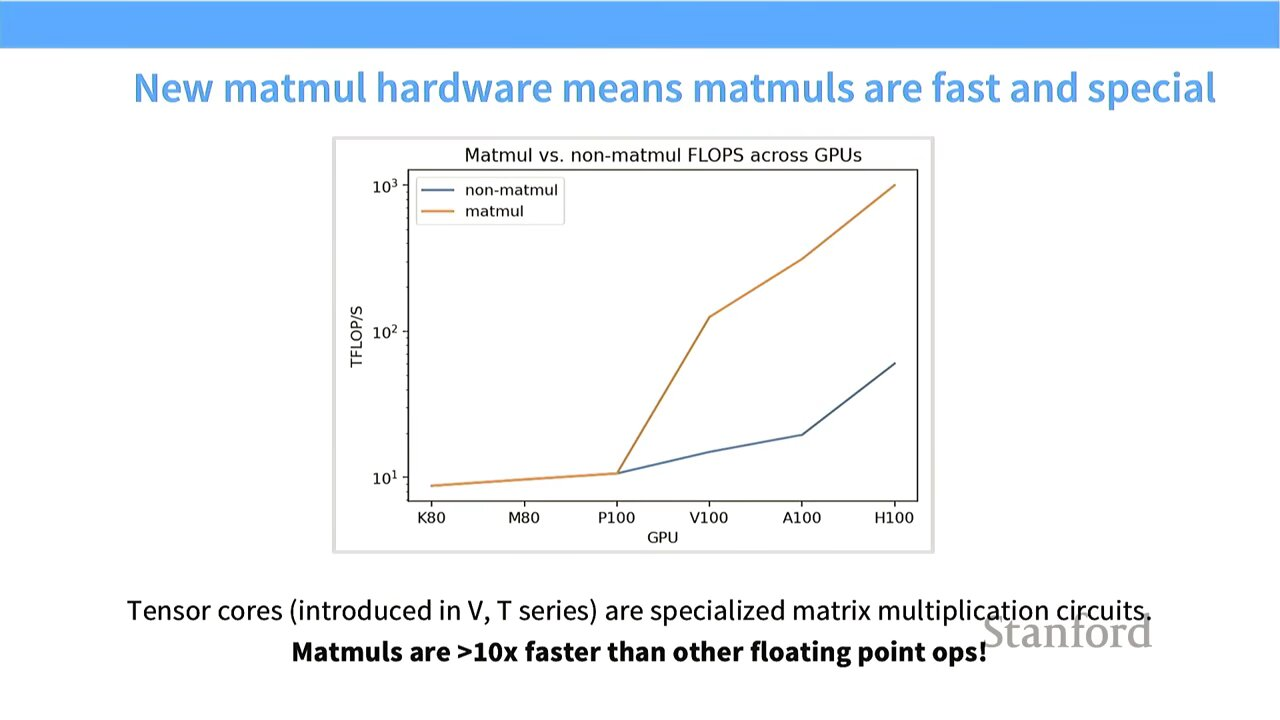
\includegraphics[width=\textwidth]{figures/fig_09_matmul_hardware.jpg}
\caption{各代 NVIDIA GPU 的 matmul TFLOPS 远超 vector TFLOPS\protect\footnotemark}
\end{figure}
\footnotetext{视频画面时间区间：00:21:00--00:21:15。}

这张图把各代 NVIDIA GPU 的 \textbf{matmul TFLOPS}（橙线，由张量核提供）和 \textbf{vector TFLOPS}（其它线，普通 ALU）画在一起。结论触目惊心：\textbf{matmul 算力随代际爆炸式增长，而普通向量算力的增长要平缓得多}。这意味着，如果你的代码能写成矩阵乘，你就能吃到 GPU 上最快的那条曲线；如果你写的是一堆逐元素的小运算，你就只能用那条慢得多的曲线。

\begin{importantbox}{一个深刻的工程启示}
\textbf{把你的计算重写成矩阵乘形式，往往是最大的性能优化。}这是 cuDNN、oneDNN、甚至 PyTorch 内部反复出现的主题。许多看似不是矩阵乘的运算（嵌入层查找、softmax、甚至排序），在底层都被改写成了矩阵乘或张量核友好的形式。
\end{importantbox}

\subsection{算力增长远快于带宽增长}

紧接着，讲师抛出了本讲最重要的趋势之一：\textbf{峰值算力（FLOPS）的增长速度，远远快于内存带宽（bytes/sec）的增长速度}。

\begin{figure}[H]
\centering
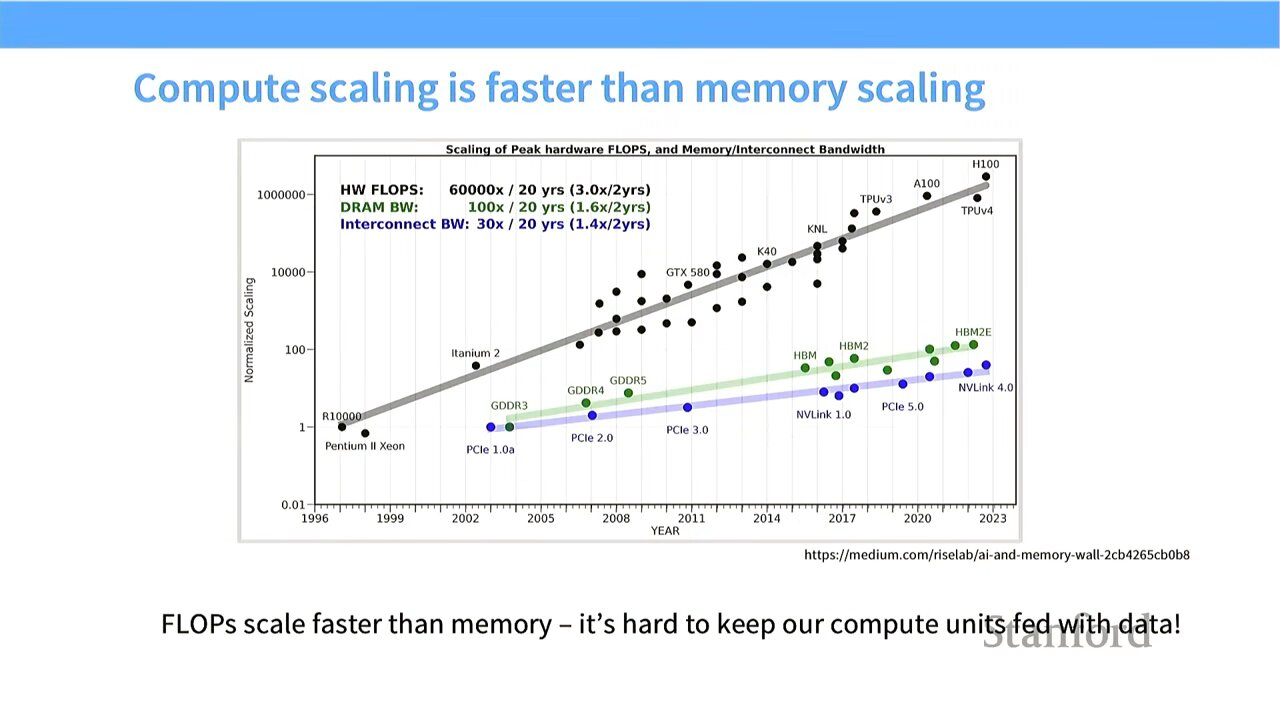
\includegraphics[width=\textwidth]{figures/fig_10_compute_vs_mem_scaling.jpg}
\caption{峰值 FLOPS 增长远快于内存/互联带宽增长\protect\footnotemark}
\end{figure}
\footnotetext{视频画面时间区间：00:22:15--00:22:30。}

这张图横轴是时间（GPU 代际），纵轴是对数尺度的性能。可以看到算力曲线的斜率明显比带宽曲线更陡。代际演进中，显存也从 GDDR 一路换到 HBM2E 再到 HBM3，带宽确实在涨，但\textbf{远远追不上算力的涨幅}。

\begin{warningbox}{趋势的后果}
每一代新 GPU，"算力 / 带宽" 这个比值都在变大。换句话说，\textbf{每个字节能养活的算力越来越多}。这意味着：那些\textbf{算术强度低}（搬一个字节只能算很少几次）的运算会越来越吃亏；只有\textbf{算术强度高}的运算才能真正用满新一代 GPU。
\end{warningbox}

\subsection{矩阵乘性能之谜}

带着上面两条趋势，讲师引出贯穿后半讲的"矩阵乘之谜"。

\begin{figure}[H]
\centering
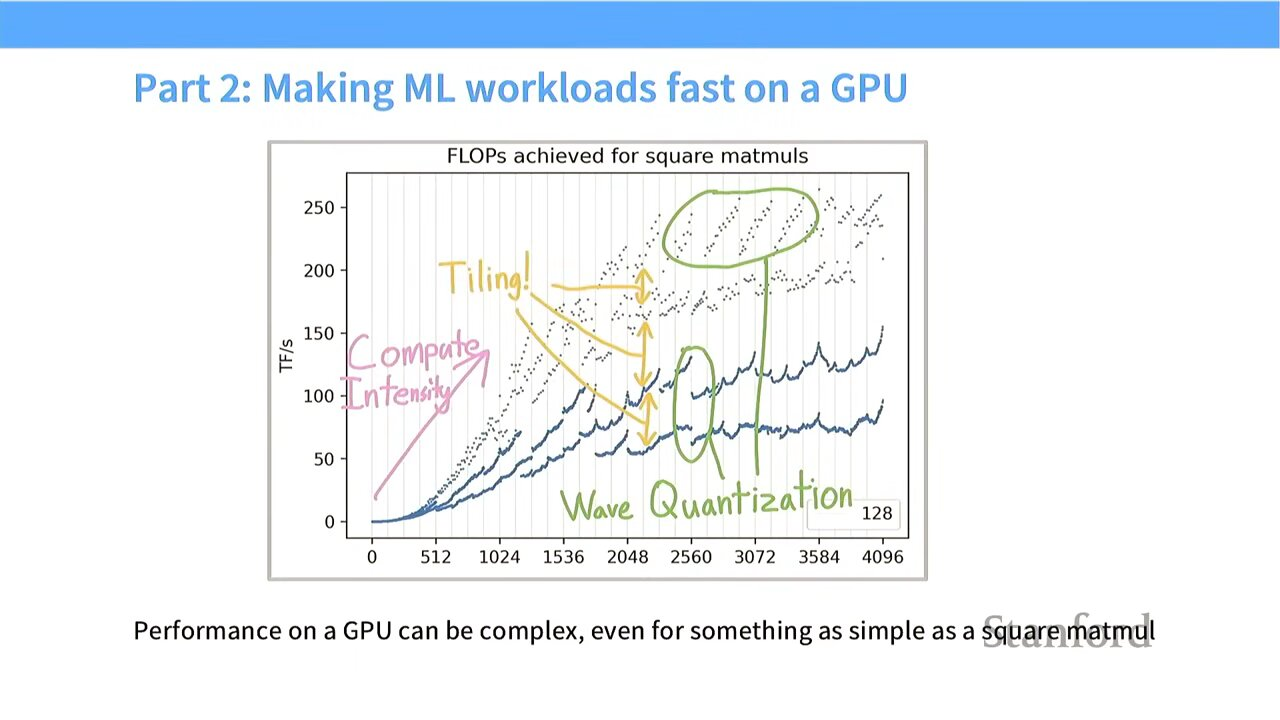
\includegraphics[width=\textwidth]{figures/fig_11_part2_mystery.jpg}
\caption{Part 2：方阵乘法的实际 TFLOPS 随尺寸呈现诡异波动\protect\footnotemark}
\end{figure}
\footnotetext{视频画面时间区间：00:25:00--00:25:15。}

横轴是方阵的尺寸 $N$，纵轴是实测的 TFLOPS。直觉上，矩阵越大算得越多，TFLOPS 应该单调上升、最后趋近硬件峰值。但实际曲线呈现\textbf{诡异的波浪形}：有快速的爬升、有突然的塌陷、有周期性的锯齿。讲师承诺，在讲完所有原理后，会回来\textbf{完整解释这张图上的每一个特征}（内存瓶颈区、分块边界、波量化）。这是本讲最强的悬念。

\subsection{Roofline 模型：算术强度决定一切}

要分析"一个运算在 GPU 上能跑多快"，最强大的工具是 \textbf{roofline 模型}。它的核心是\textbf{算术强度（arithmetic intensity）}的定义：

\[
\text{arithmetic intensity} = \frac{\text{FLOPs performed}}{\text{bytes accessed}}
\]

即"每搬运一个字节，能做多少次浮点运算"。单位是 FLOPs/byte。算术强度高的运算倾向于\textbf{计算受限（compute-bound）}，低的倾向于\textbf{内存受限（memory-bound）}。

\begin{figure}[H]
\centering
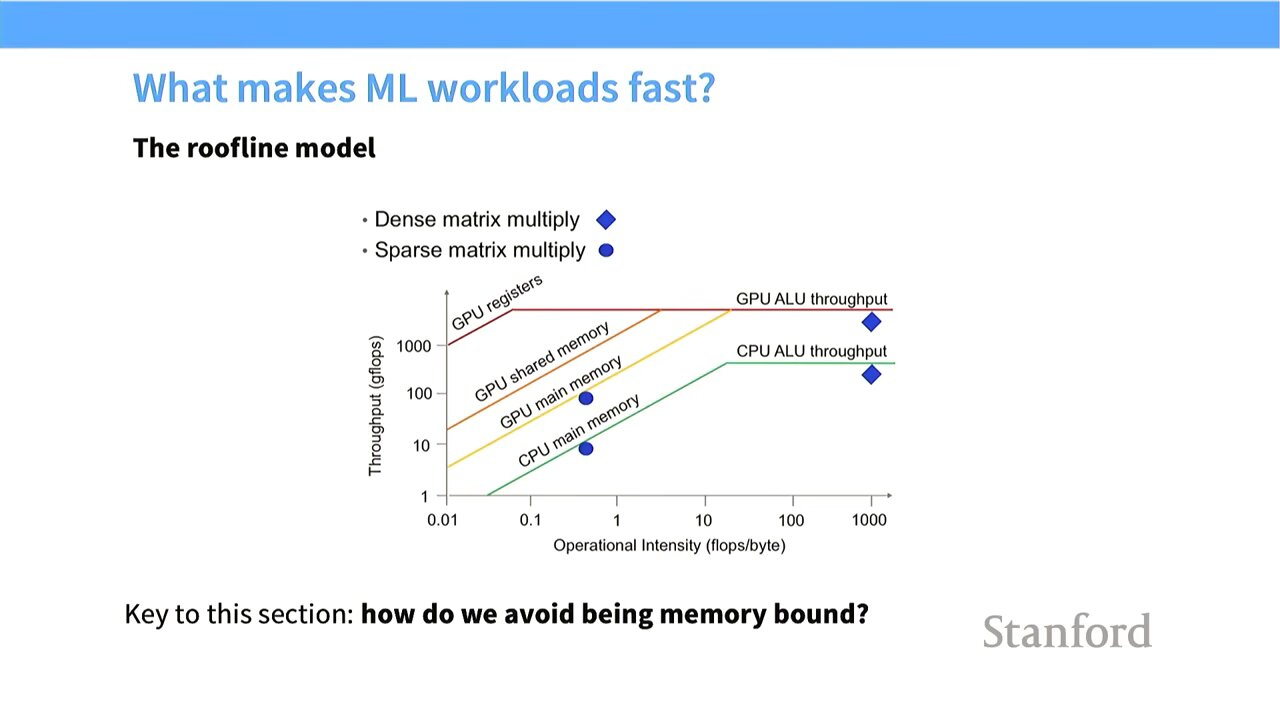
\includegraphics[width=\textwidth]{figures/fig_12_roofline.jpg}
\caption{Roofline 模型：吞吐由内存带宽与峰值算力两条线共同决定\protect\footnotemark}
\end{figure}
\footnotetext{视频画面时间区间：00:26:30--00:26:45。}

roofline 图的横轴是算术强度（FLOPs/byte，对数尺度），纵轴是可达吞吐（GFLOPs/s，对数尺度）。图上有两条关键的"屋顶"线：

\begin{itemize}
\item \textbf{内存带宽线（斜率为正的部分）}：在算术强度较低时，吞吐受限于"能搬多少字节"。公式为 $\text{Throughput} = \text{arithmetic intensity} \times \text{bandwidth}$，在对数图上是一条斜率为 1 的直线。
\item \textbf{峰值算力线（水平部分）}：当算术强度足够高，搬数据不再是瓶颈，吞吐被峰值 FLOPS 封顶，是一条水平线。
\end{itemize}

两条线的交点对应的算术强度，叫做 \textbf{脊点（ridge point）}：

\[
\text{ridge point} = \frac{\text{peak FLOPS}}{\text{peak bandwidth}}
\]

\begin{knowledgebox}{如何用 roofline 判断瓶颈}
把你的运算的算术强度标到 roofline 图上：
\begin{itemize}
\item 若落在斜线段（运算点左侧），你是\textbf{内存受限}，优化方向是\textbf{减少访存或提高算术强度}。
\item 若落在水平段（运算点右侧），你是\textbf{计算受限}，优化方向是\textbf{降低精度、用张量核}。
\end{itemize}
这个判断决定了你应该优先做哪种优化，是本讲最重要的方法论。
\end{knowledgebox}

\section{SIMT 与控制流分叉}

在讲优化技巧之前，讲师补充了一个执行层面的重要现象：\textbf{控制流分叉（control divergence）}，它源于 SIMT 模型。

\begin{figure}[H]
\centering
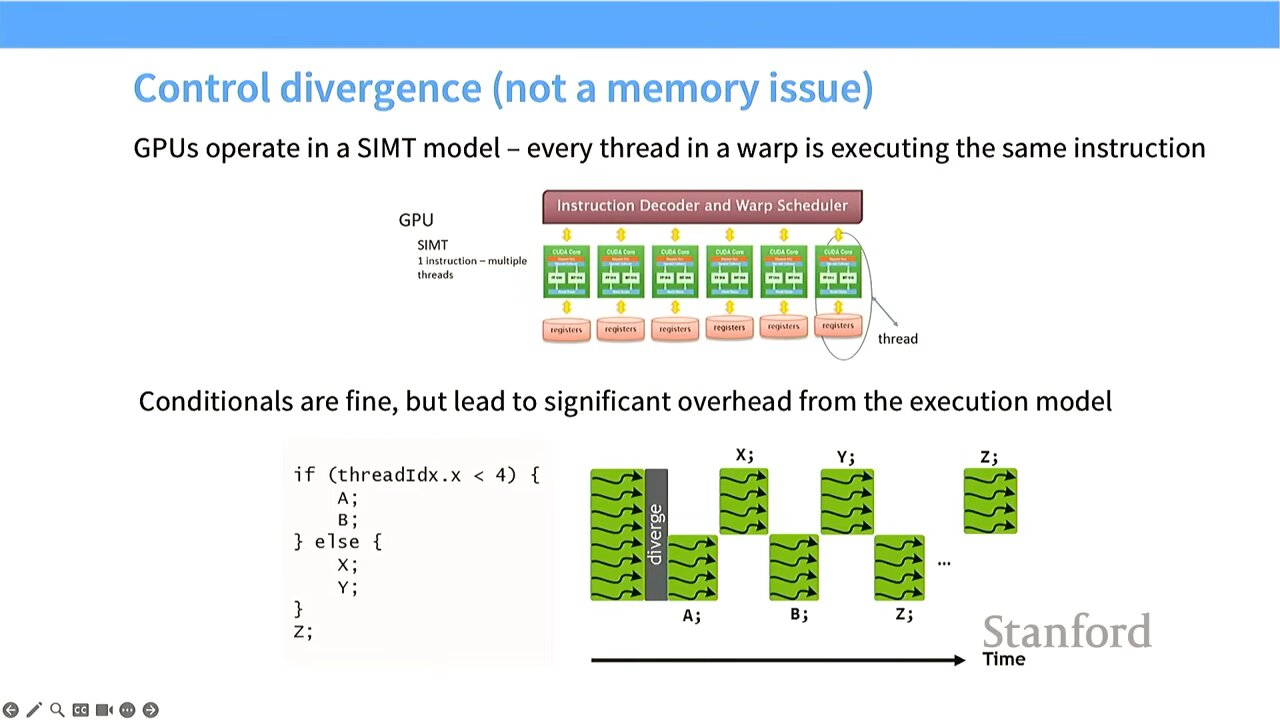
\includegraphics[width=\textwidth]{figures/fig_13_control_divergence.jpg}
\caption{warp 内不同线程走不同分支会导致分叉（串行化）\protect\footnotemark}
\end{figure}
\footnotetext{视频画面时间区间：00:28:15--00:28:30。}

回顾 SIMT：一个 warp 的 32 个线程在同一周期执行\textbf{同一条}指令。那如果代码里有 \texttt{if/else} 分支怎么办？比如：

\begin{lstlisting}[language=C++]
if (x < 0) {
    y = 0;          // then branch
} else {
    y = x;          // else branch
}
\end{lstlisting}

如果一个 warp 内有的线程满足 $x<0$、有的不满足，硬件无法让它们同时走不同分支。实际发生的是\textbf{串行化}：硬件先让满足 then 分支的线程执行（其余线程空闲等待），再让满足 else 分支的线程执行（先前那批反过来等待）。两条分支都被完整执行了一遍，只是各自只有一半线程在干活。

\begin{warningbox}{warp divergence 的代价}
分叉本身\textbf{不是内存问题，而是执行效率问题}：分支越多、warp 内分歧越严重，实际吞吐越低。最坏情况下，一个含 $k$ 条互斥分支的 warp，相当于把吞吐砍到 $1/k$。
\end{warningbox}

实践上，应尽量保证同一 warp 内的线程走相同的控制流路径，例如按数据特征对线程做排序/分组，或把发散的分支重排成无分支的位运算。

\section{让 ML 负载变快的五大技巧}

讲师接下来系统地介绍了让 ML 负载在 GPU 上跑得更快的五大技巧。这五个技巧本质都在做同一件事：\textbf{用 GPU 上相对充裕的资源（算力）去换取相对稀缺的资源（内存带宽）}。

\subsection{技巧 1：低精度计算}

第一个技巧最直接：\textbf{降低数据精度}。从 FP32 一路降到 FP16、BF16、FP8、INT8，每个数值占的字节数减半，等效带宽和算力都翻倍。

\begin{figure}[H]
\centering
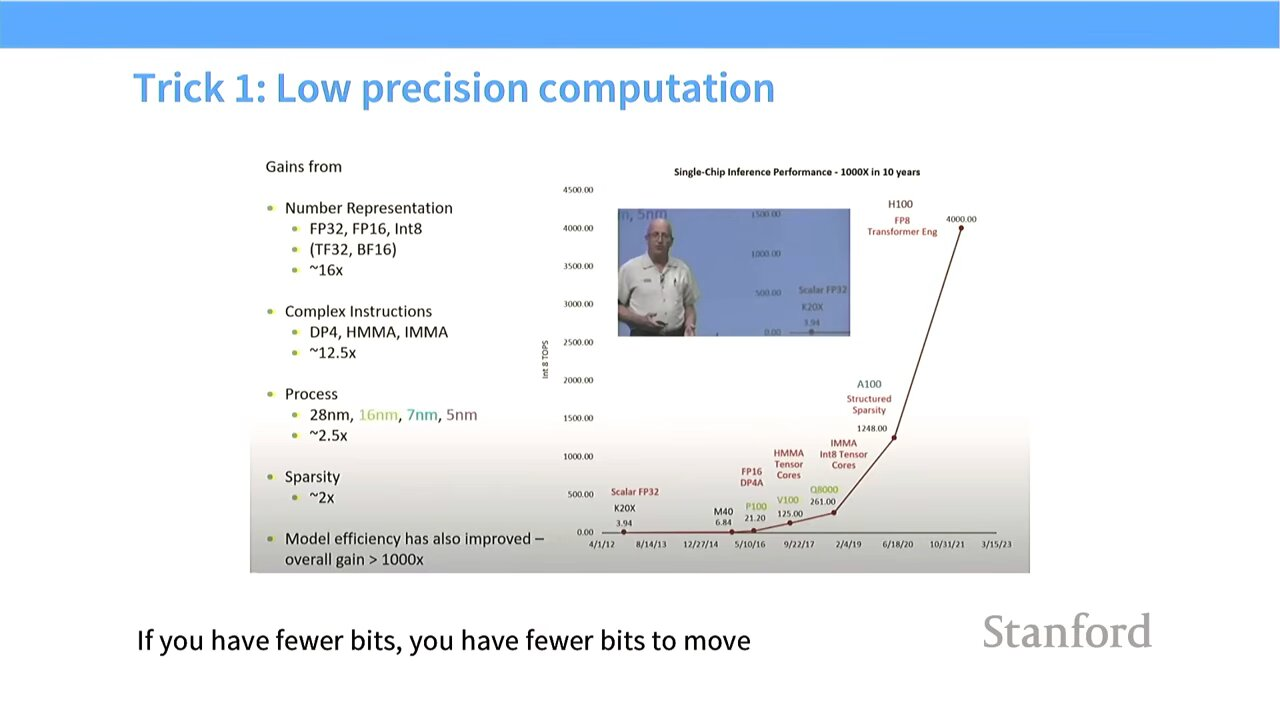
\includegraphics[width=\textwidth]{figures/fig_14_low_precision.jpg}
\caption{技巧 1：单芯片推理性能十年提升 1000 倍，精度下降是主因之一\protect\footnotemark}
\end{figure}
\footnotetext{视频画面时间区间：00:29:45--00:30:00。}

讲师展示了一张"单芯片推理性能十年提升 1000 倍"的图，其中精度降低（FP32 $\to$ FP16 $\to$ INT8 $\to$ ...）贡献了相当一部分。精度层级的演进大致是：

\[
\text{FP32} \;\to\; \text{FP16} \;\to\; \text{BF16} \;\to\; \text{INT8} \;\to\; \text{FP4/INT4}
\]

关键在于：\textbf{张量核针对低精度做了专门的硬件加速}。以矩阵乘为例，输入可以用 FP16/BF16，但\textbf{累加在 FP32 里完成}，兼顾速度与数值稳定性：

\[
\text{acc}_{ij} \mathrel{+}= A_{ik} \cdot B_{kj}, \qquad A,B \in \text{FP16},\; \text{acc} \in \text{FP32}
\]

用带宽衡量，从 FP32 降到 FP16 等效带宽翻倍：

\[
\text{effective bandwidth}(\text{FP16}) = 2 \times \text{effective bandwidth}(\text{FP32})
\]

进一步降到 INT8 则再翻倍。这就是为什么每次精度下降一档，roofline 的脊点也会左移——同样的硬件可以处理算术强度更低的负载。

\begin{importantbox}{BF16 vs FP16}
BF16（brain float 16）保留了 FP32 的 8 位指数，只牺牲尾数位数，因此\textbf{动态范围与 FP32 相同}，训练时不容易溢出，成为现代 LLM 训练的事实标准。FP16 指数位少，范围窄，容易在中间激活值上溢出。这是为什么 BF16 在大模型里更受青睐。
\end{importantbox}

\subsection{技巧 2：算子融合}

第二个技巧是\textbf{算子融合（operator fusion）}。回顾前面"算力涨得比带宽快"，意味着\textbf{每次把数据搬进搬出 HBM 都很昂贵}。如果两个算子是串联的（前一个的输出是后一个的输入），把中间结果写回 HBM 再读回来，就是浪费。

\begin{figure}[H]
\centering
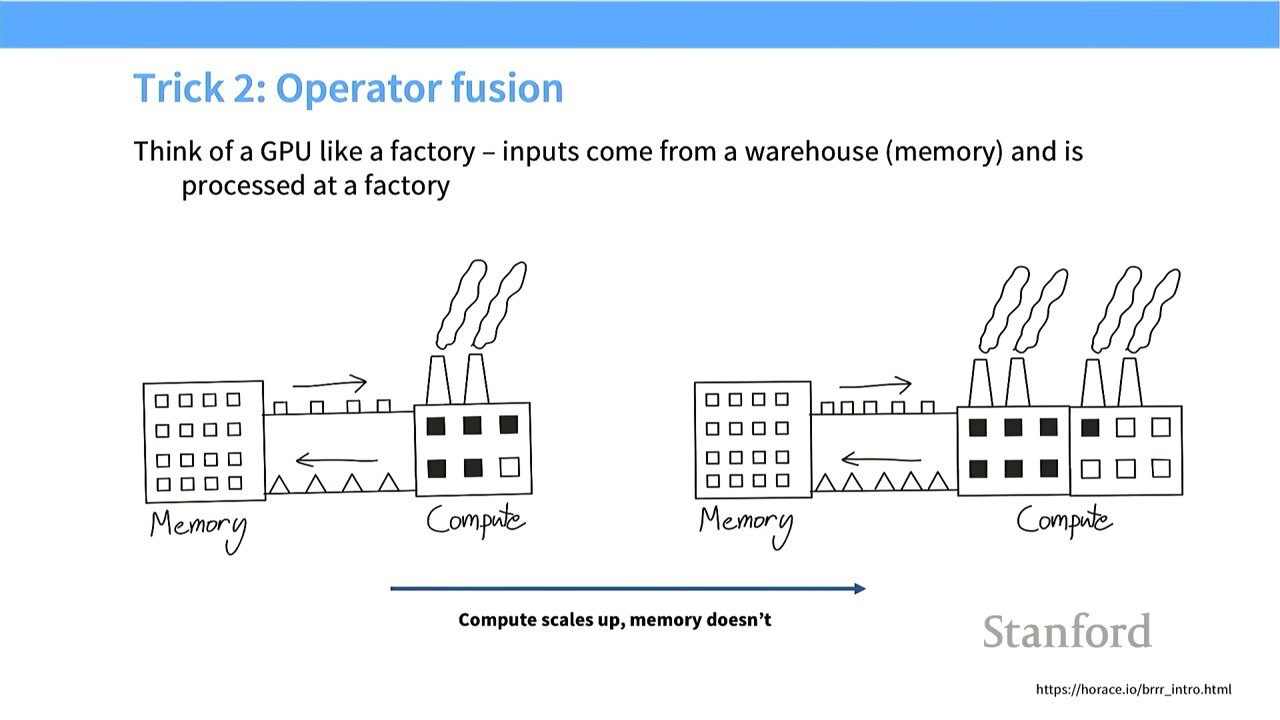
\includegraphics[width=\textwidth]{figures/fig_15_operator_fusion_factory.jpg}
\caption{技巧 2：算子融合——把"工厂"（计算）和"仓库"（内存）合在一起\protect\footnotemark}
\end{figure}
\footnotetext{视频画面时间区间：00:33:30--00:33:45。}

讲师用一个非常贴切的\textbf{工厂类比}：把 GPU 想象成一个工厂，计算单元是"车间"，内存是"仓库"。算力（车间产能）在不断扩张，而带宽（仓库到车间的传送带）扩张缓慢。如果每道工序都把半成品送回仓库、下一道工序再从仓库取出来，传送带就成了瓶颈。算子融合就是\textbf{把多道工序合并成一个车间内的流水线}，半成品全程不落地、不进仓库。

形式化地说，未融合时：

\[
y = g(f(x)) \;\Rightarrow\; t = f(x)\;(\text{写 HBM}),\;\; y = g(t)\;(\text{读 HBM})
\]

融合后：

\[
y = g(f(x)) \;\Rightarrow\; \text{在寄存器/共享内存里直接 } y = g(f(x))\text{，零次 HBM 读写}
\]

对比两者的算术强度。设 $f, g$ 各做 $c_f, c_g$ 次运算、操作的字节数为 $b$。未融合时三个 kernel 的综合算术强度为：

\[
\text{AI}_{\text{unfused}} = \frac{c_f + c_g}{3b}
\]

（一次读入、一次写出中间结果、一次读回，共约 $3b$ 字节搬运）。融合后中间结果不落地：

\[
\text{AI}_{\text{fused}} = \frac{c_f + c_g}{b}
\]

算术强度直接提升 3 倍，这往往足以把负载从内存受限的斜线段推到计算受限的水平段。

\begin{figure}[H]
\centering
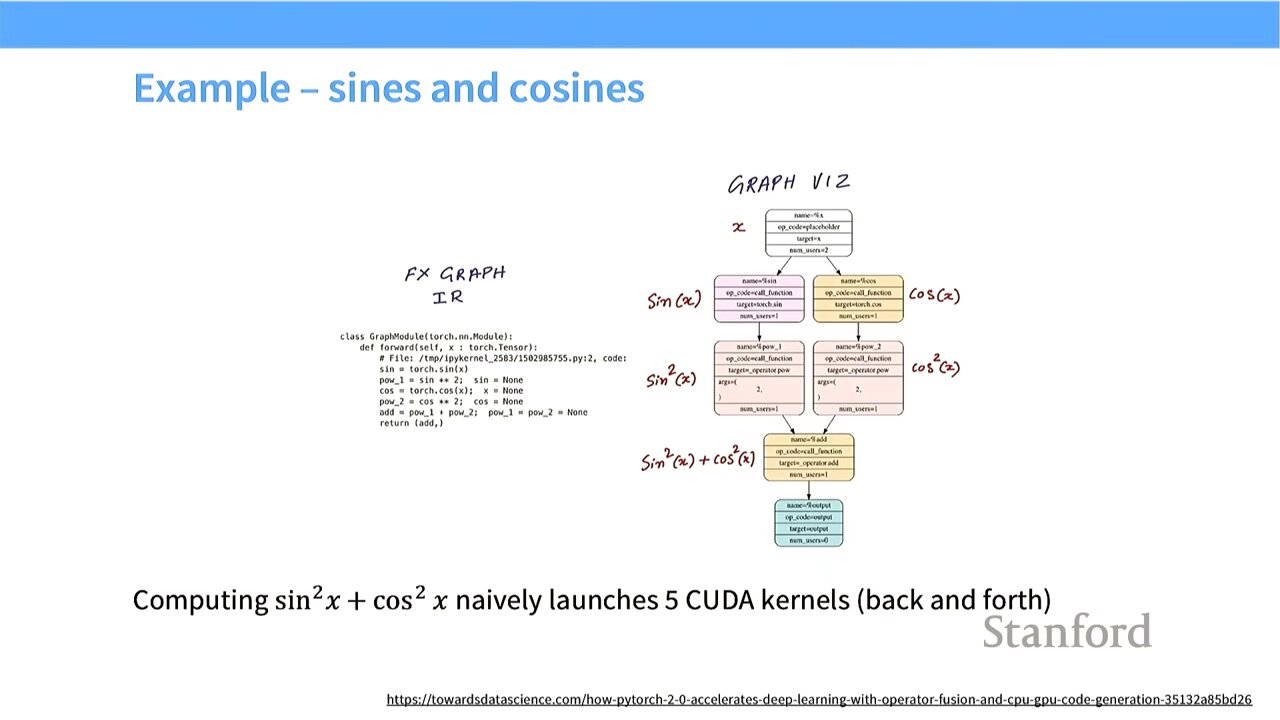
\includegraphics[width=\textwidth]{figures/fig_16_fused_sincos.jpg}
\caption{技巧 2 实例：融合 sin/cos，一次访算出两个值\protect\footnotemark}
\end{figure}
\footnotetext{视频画面时间区间：00:35:15--00:35:30。}

讲师以 \texttt{sin} 和 \texttt{cos} 为例：很多场景（如位置编码 RoPE）要同时算 $\sin(x)$ 和 $\cos(x)$。分开写就是两个 kernel、两次读 $x$。融合成一个 \texttt{sincos} kernel 后，$x$ 只读一次，$\sin$ 和 $\cos$ 在寄存器里同时算出。PyTorch 2.0 的 \texttt{torch.compile} 就是在做这种自动算子融合——它把 Python 定义的计算图编译成一连串融合好的 CUDA kernel。

\begin{practicebox}{torch.compile 的本质}
\texttt{torch.compile}（以及 Triton、JAX 的 XLA）的核心价值之一就是\textbf{自动算子融合}：把相邻的逐元素算子、激活函数、类型转换等合并成单个 kernel，大幅减少 HBM 往返。在 LLM 训练里，开启 \texttt{torch.compile} 经常能拿到两位数百分比的提速，几乎不用改业务代码。
\end{practicebox}

\subsection{技巧 3：重计算（梯度检查点）}

第三个技巧看似反直觉：\textbf{主动丢弃前向的中间激活值，反向时再重新算一遍}。这叫\textbf{重计算（recomputation）}，也常被称为\textbf{梯度检查点（gradient checkpointing）}。

\begin{figure}[H]
\centering
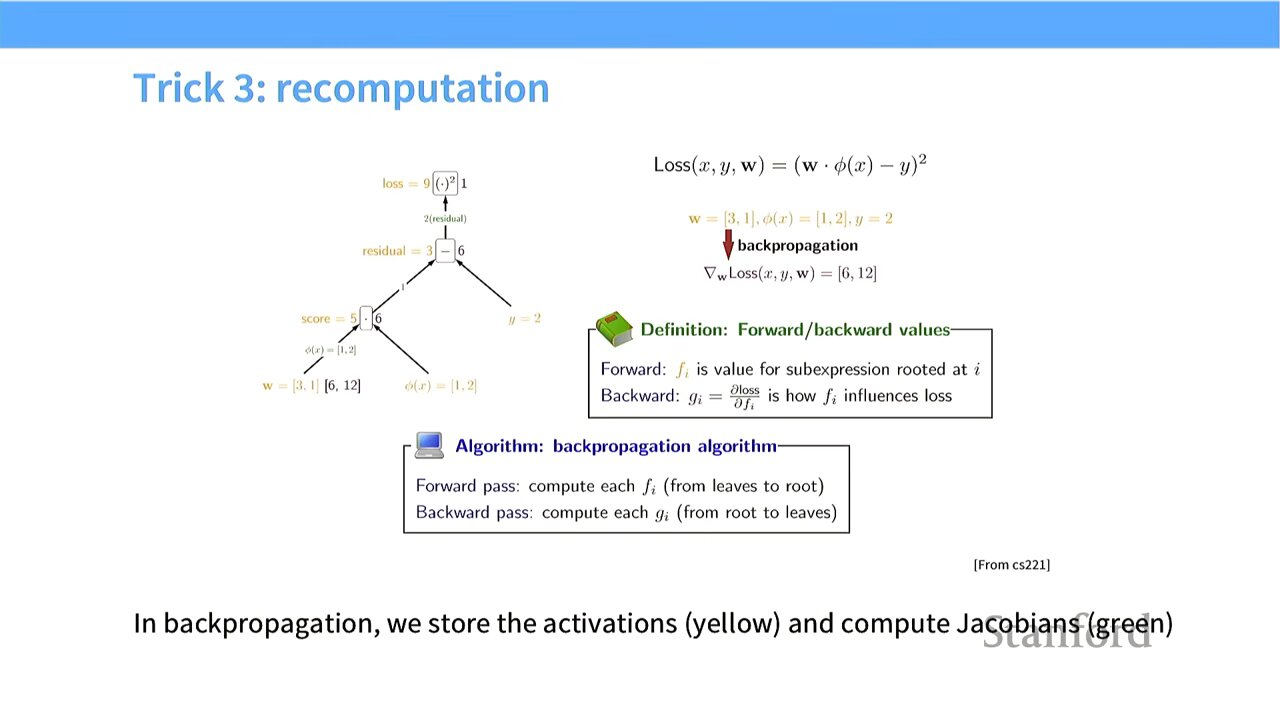
\includegraphics[width=\textwidth]{figures/fig_17_recomputation_backprop.jpg}
\caption{技巧 3：反向传播中按需重算激活，用算力换显存\protect\footnotemark}
\end{figure}
\footnotetext{视频画面时间区间：00:37:30--00:37:45。}

回顾反向传播：要计算梯度，需要用到前向时的中间激活值。常规做法是把所有中间激活存起来——但激活值随序列长度和模型规模线性甚至二次增长，很快就把显存撑爆。重计算的做法是：前向时\textbf{只存少量检查点}（比如每层的输入），把逐层的中间激活丢弃；反向时，从最近的检查点出发，\textbf{重新前向计算}所需的激活。

\begin{figure}[H]
\centering
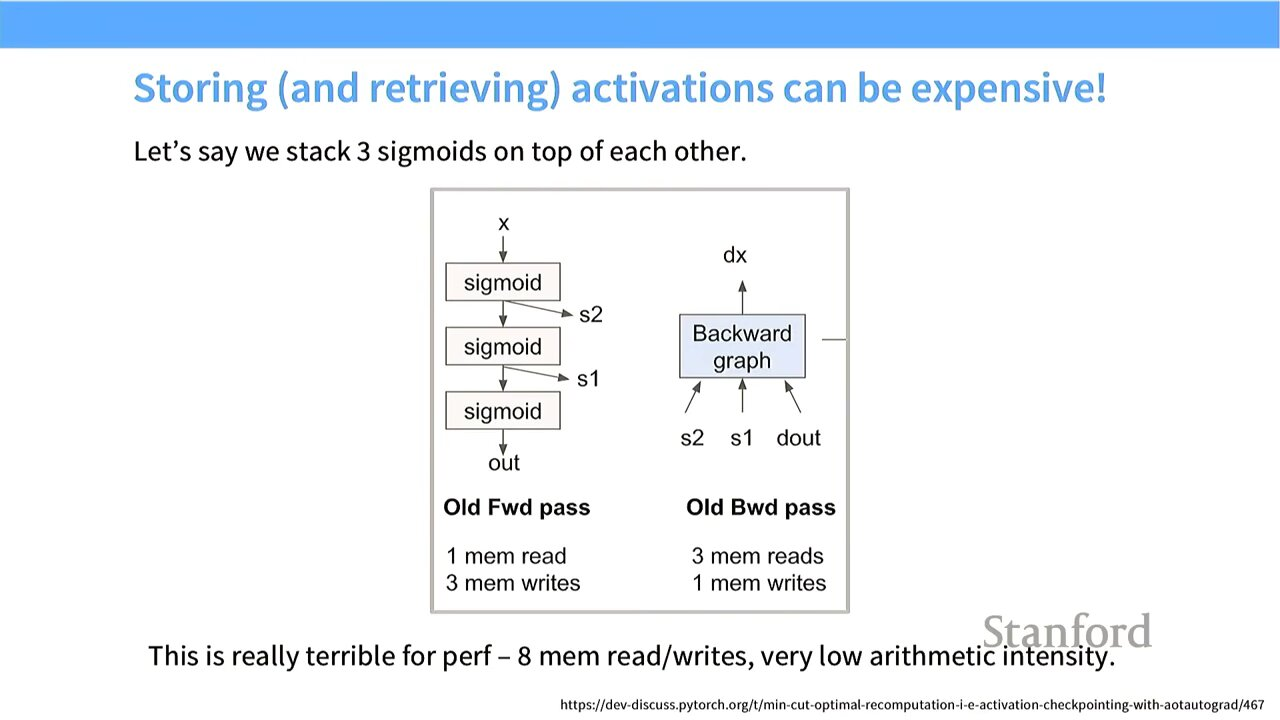
\includegraphics[width=\textwidth]{figures/fig_18_recomputation_sigmoid.jpg}
\caption{技巧 3 实例：sigmoid 的激活可由输出廉价重建\protect\footnotemark}
\end{figure}
\footnotetext{视频画面时间区间：00:38:45--00:39:00。}

讲师用 sigmoid 举了一个特别优雅的例子。sigmoid 函数 $\sigma(x) = \frac{1}{1+e^{-x}}$ 的导数有一个美妙性质：

\[
\sigma'(x) = \sigma(x)\,(1 - \sigma(x))
\]

也就是说，\textbf{只要保存了前向输出 $\sigma(x)$，就能用上式直接算出导数，完全不需要保存前向输入 $x$}。这意味着对于 sigmoid，激活值可以"免费"重建——存输出就够了。这本质上就是一种自然的重计算。

\begin{knowledgebox}{重计算的本质：算力换显存}
回顾 roofline：算力相对充裕（计算受限少），而显存带宽与容量都紧张。重计算就是\textbf{用充裕的算力去节省稀缺的显存}。代价是反向时多一次前向计算（约 30\% 计算开销），换来的是激活显存从 $O(L)$ 降到 $O(\sqrt{L})$（$L$ 为层数），让大模型训练成为可能。这是一笔非常划算的交易。
\end{knowledgebox}

形式化地，朴素反向传播需要保存每层激活，显存开销为：

\[
\text{memory}_{\text{naive}} = O(L \cdot d \cdot N)
\]

其中 $L$ 是层数、$d$ 是隐藏维度、$N$ 是序列长度。采用梯度检查点后，只保存 $\sqrt{L}$ 个检查点，每段重计算，显存降为：

\[
\text{memory}_{\text{checkpoint}} = O(\sqrt{L} \cdot d \cdot N)
\]

代价是反向多了一次前向计算，总计算量从 $2\times$（一次前向 + 一次反向）变为约 $2.33\times$。

\subsection{技巧 4：内存合并、突发模式与缓存}

第四个技巧关于\textbf{访存模式}。GPU 访问全局内存时，并不是"要一个字节取一个字节"，而是以更大的粒度批量搬运，叫做 \textbf{突发模式（burst mode）}或突发段（burst section）。

\begin{figure}[H]
\centering
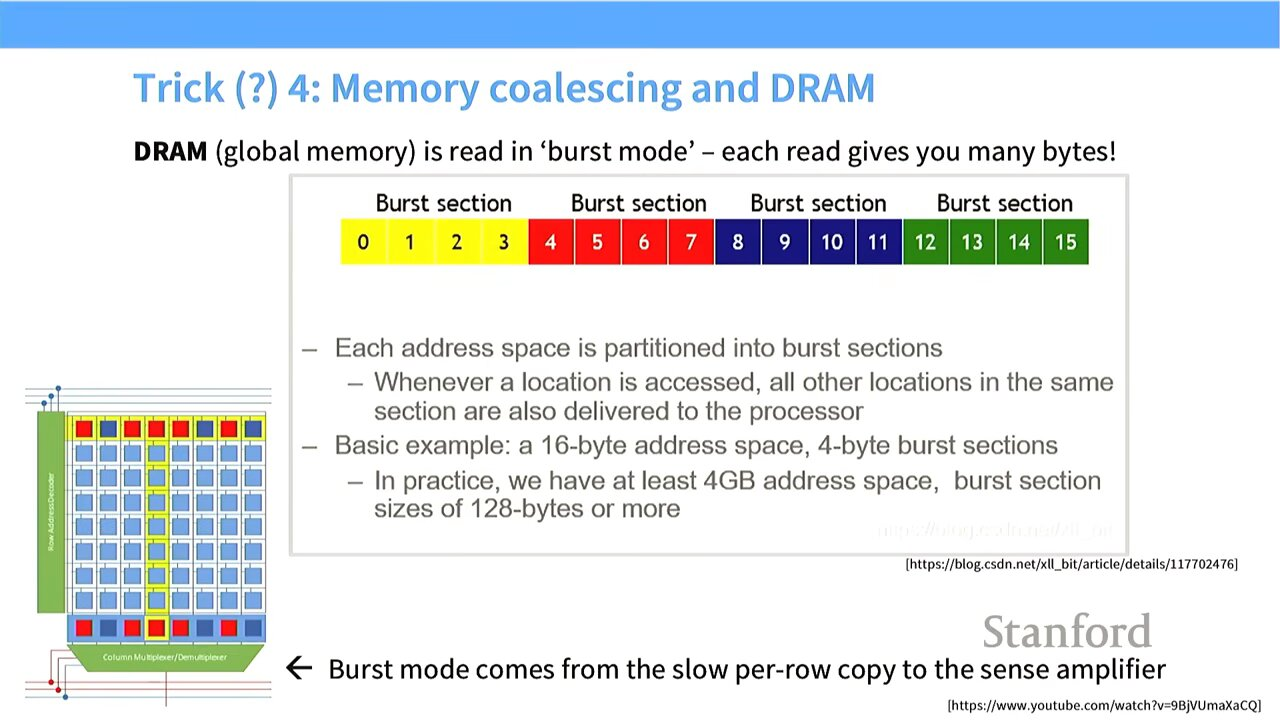
\includegraphics[width=\textwidth]{figures/fig_19_memory_coalescing.jpg}
\caption{技巧 4：内存合并——连续地址的访问被合并成一次突发传输\protect\footnotemark}
\end{figure}
\footnotetext{视频画面时间区间：00:41:30--00:41:45。}

当一个 warp 的 32 个线程\textbf{访问连续的内存地址}时（比如线程 $i$ 访问第 $i$ 个 4 字节浮点数），硬件会把这些访问\textbf{合并（coalesce）}成一次突发传输，效率极高。反之，如果 32 个线程访问的是分散的、不连续的地址，硬件不得不发起多次传输，吞吐暴跌。

\begin{warningbox}{跨步访问的代价}
假设 warp 内线程访问的是 \texttt{array[stride * tid]}，stride 很大且不连续。这种\textbf{跨步（strided）或随机访问}会让合并失败，每个线程的访问都触发独立的内存事务，实测带宽可能降到合并访问的 $1/10$ 以下。这是很多 GPU kernel 性能不及预期的头号原因。
\end{warningbox}

更微妙的是\textbf{突发段与分块的对齐}问题。如果矩阵布局里，分块的起始位置没有和突发段边界对齐（比如多了 1 个元素），那么原本一次能取完的一行，会被迫拆成两次突发传输——仅仅因为多了一个元素，访存量直接翻倍。解决方法是\textbf{padding}：把矩阵尺寸补齐到突发段大小的整数倍。这个细节会在后面"波量化与 padding"一节再次出现。

\begin{practicebox}{合并访问的编程准则}
写 kernel 时，务必让 warp 内的线程访问\textbf{地址连续}的数据。在存储矩阵时，让最内层维度是连续的（row-major 下沿列访问要注意），并尽量让分块大小是 32 的倍数（与 warp 对齐）。这些都是无形的性能开关。
\end{practicebox}

\subsection{技巧 5：分块（Tiling）}

第五个、也是最重要最复杂的技巧：\textbf{分块（tiling）}。它把"搬到共享内存重用"和"内存合并"两条思路合二为一，是高性能矩阵乘的核心。

\begin{figure}[H]
\centering
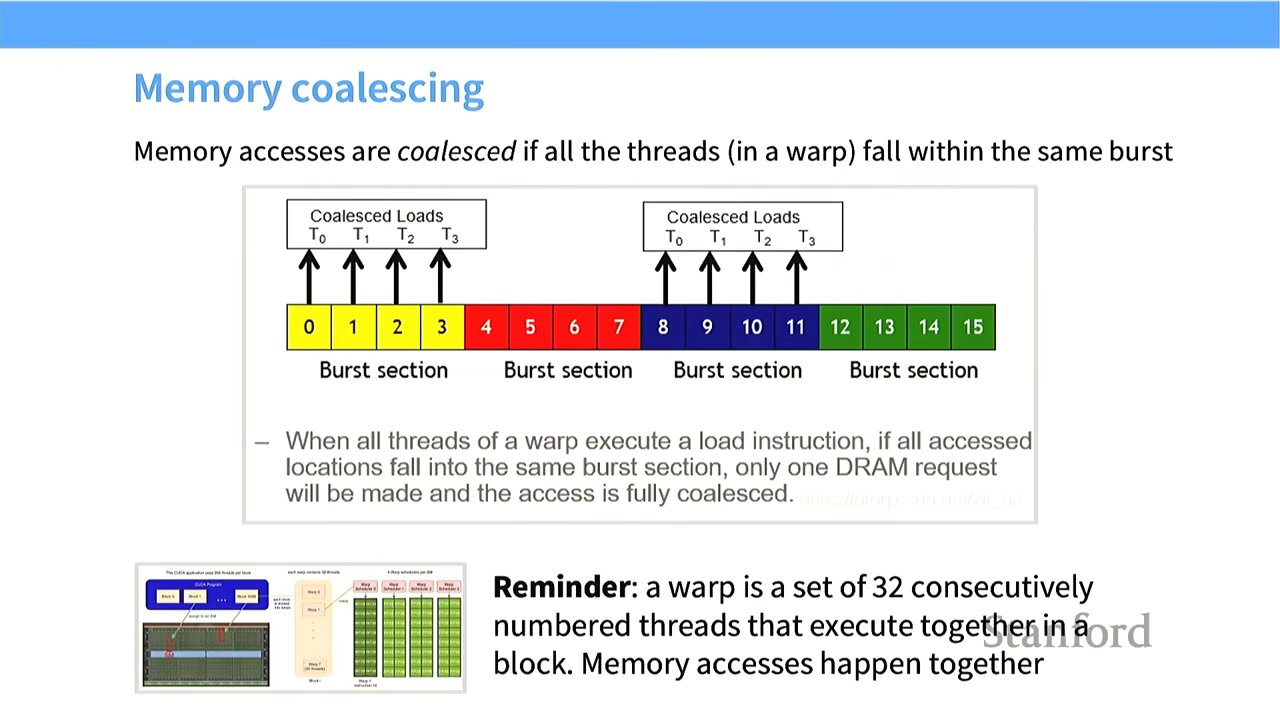
\includegraphics[width=\textwidth]{figures/fig_20_tiling_intro.jpg}
\caption{技巧 5：分块——把大矩阵切成小块搬到共享内存\protect\footnotemark}
\end{figure}
\footnotetext{视频画面时间区间：00:43:45--00:44:00。}

考虑矩阵乘 $C = A \times B$，三者都是 $N \times N$。朴素的实现里，每计算 $C$ 的一个元素，都要读 $A$ 的一整行和 $B$ 的一整列；而 $A$ 的每个元素会被读 $N$ 次（每个 $C$ 的元素都要用它一次），全部来自慢速全局内存。

\begin{figure}[H]
\centering
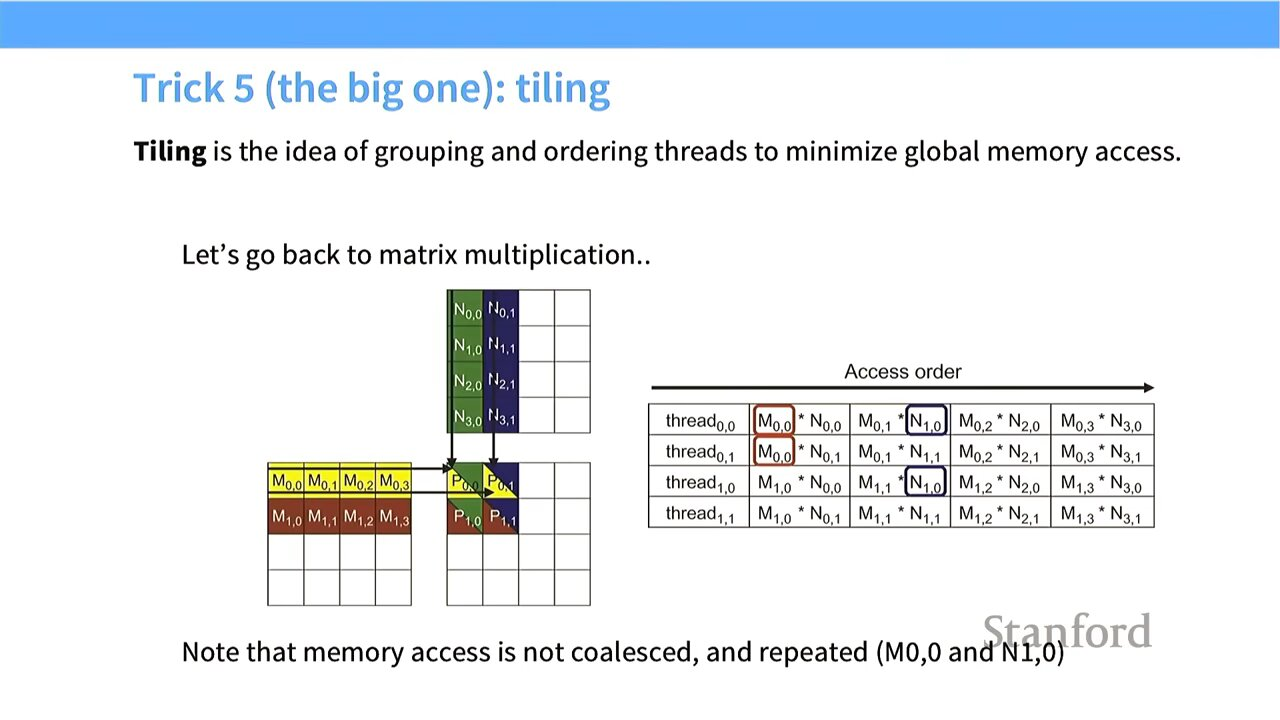
\includegraphics[width=\textwidth]{figures/fig_21_tiling_loop_reorder.jpg}
\caption{技巧 5：循环重排让内存访问模式变得连续可合并\protect\footnotemark}
\end{figure}
\footnotetext{视频画面时间区间：00:46:45--00:47:00。}

分块的做法是：把 $A,B,C$ 都切成大小为 $T \times T$ 的小块。计算时，先把一个 $A$ 的块和一个 $B$ 的块\textbf{从全局内存搬到共享内存}，然后让对应 block 的所有线程\textbf{在共享内存里}反复读这两个块、累加到 $C$ 的块上。搬进共享内存后，后续的 $T$ 次重用全部走快速共享内存。

\begin{figure}[H]
\centering
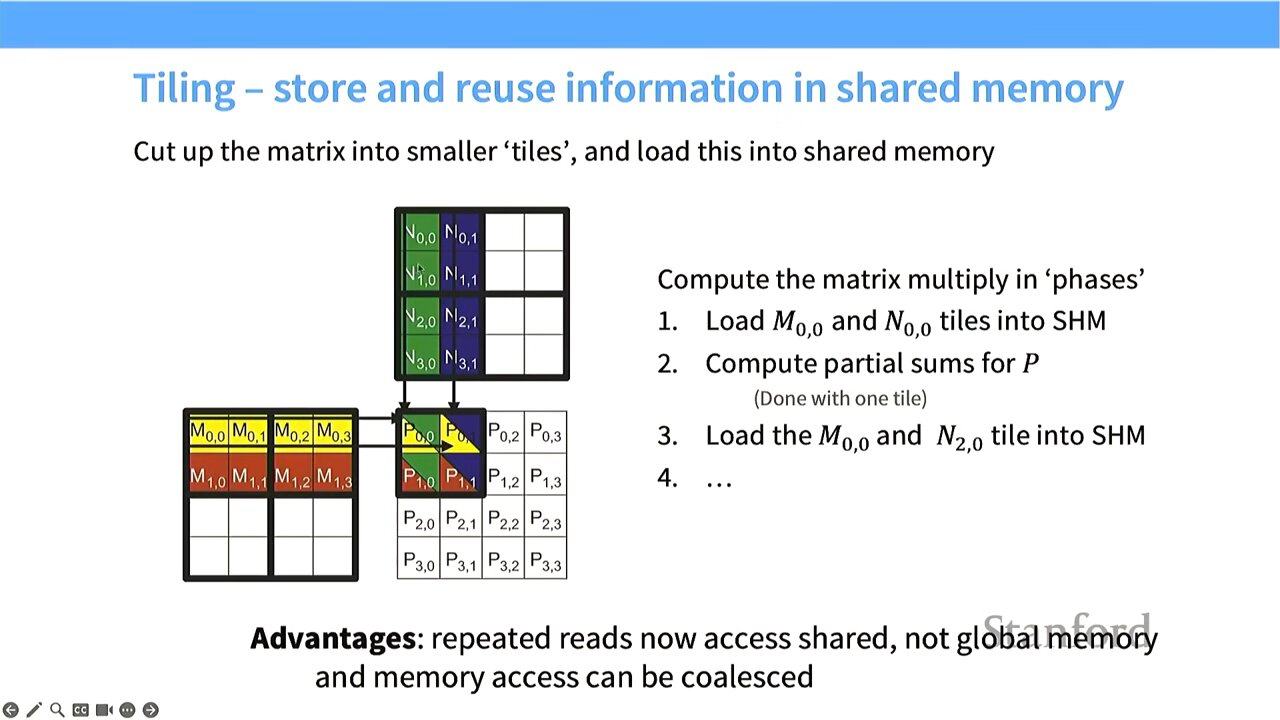
\includegraphics[width=\textwidth]{figures/fig_22_tiling_analysis.jpg}
\caption{技巧 5：分块前后的全局访存量对比\protect\footnotemark}
\end{figure}
\footnotetext{视频画面时间区间：00:49:45--00:50:00。}

讲师给出了一组简洁的\textbf{分块数学}。设矩阵大小为 $N$，分块大小为 $T$：

\begin{itemize}
\item \textbf{不分块}：每个输入元素从全局内存被读 $N$ 次。
\item \textbf{分块}：每个输入元素从全局内存被读 $N/T$ 次，其余 $T$ 次重用都发生在共享内存里。
\end{itemize}

也就是说，分块把全局内存的读取量降低了\textbf{一个因子 $T$}：

\[
\text{global reads}_{\text{tiled}} = \frac{N}{T} \times \text{global reads}_{\text{naive}}, \qquad T \text{ 越大越好（受共享内存容量限制）}
\]

更精确地，朴素实现的每元素全局读次数和分块后的对比为：

\[
\text{reads per element}_{\text{naive}} = N, \qquad \text{reads per element}_{\text{tiled}} = \frac{N}{T}
\]

这正是分块能在 roofline 上把负载从内存受限推向计算受限的根本原因——它在不改变总计算量的前提下，大幅提高了有效算术强度。

\begin{importantbox}{分块的硬约束}
$T$ 不能无限大——共享内存容量有限（每个 SM 通常几十 KB）。而且分块还要兼顾\textbf{内存合并}（块大小要和突发段对齐）和\textbf{波量化}（块数要能整除矩阵维度）。这些约束相互牵扯，让 tiling 成为 GPU 编程里最"艺术"的部分。
\end{importantbox}

\section{波量化与 padding}

\subsection{波量化：尺寸不对齐导致的吞吐塌陷}

分块引出了一个非常重要的性能现象：\textbf{波量化（wave quantization）}。它的本质是——\textbf{当工作量不能正好填满 GPU 的 SM 时，会有 SM 闲置，吞吐突然掉一截}。

\begin{figure}[H]
\centering
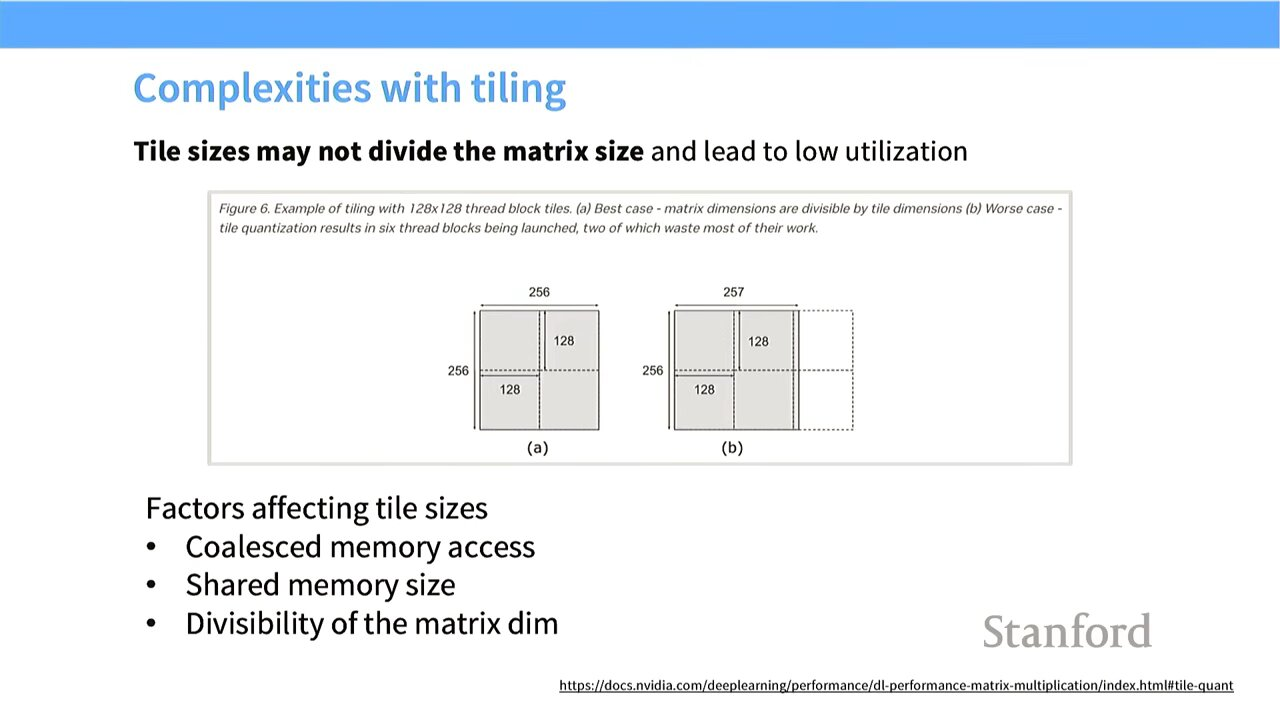
\includegraphics[width=\textwidth]{figures/fig_23_wave_quant_257.jpg}
\caption{波量化：尺寸从 256 到 257 时，第六个 tile 几乎全空，SM 闲置\protect\footnotemark}
\end{figure}
\footnotetext{视频画面时间区间：00:53:45--00:54:00。}

讲师用一个具体例子说明。设 tile size 为 128。当矩阵尺寸恰好是 256 时，正好分成 $2 \times 2$ 共 4 个完整的 tile，每个 tile 分配给一个 SM，大家都有充足的工作，负载均衡。但如果矩阵尺寸是 \textbf{257} 呢？为了覆盖多出来的 1 列，需要在列方向上多分出一个 tile，于是总共有 $2 \times 3 = 6$ 个 tile。可右边那一列的 2 个 tile \textbf{几乎是空的}——每个只有 $128 \times 1$ 的有效数据。这 2 个 tile 也会各占一个 SM，但那个 SM 99\% 的时间都在闲置。这就是波量化导致的吞吐塌陷。

\begin{warningbox}{波量化的微观机制}
GPU 的工作以"波（wave）"为单位调度：一波 = 能同时占满所有 SM 的 tile 集合。如果工作量是 $k$ 波 + 一个不完整的尾波，那个尾波会让所有 SM 都只做了一点点就结束，相当于\textbf{整波的时间只产出了尾波的工作量}，吞吐断崖式下跌。
\end{warningbox}

\subsection{矩阵乘之谜的完整解释}

带着内存瓶颈、分块、波量化、padding 这些概念，讲师终于回到前面那张神秘的"实测 TFLOPS vs 矩阵尺寸"图，逐段拆解。

\begin{figure}[H]
\centering
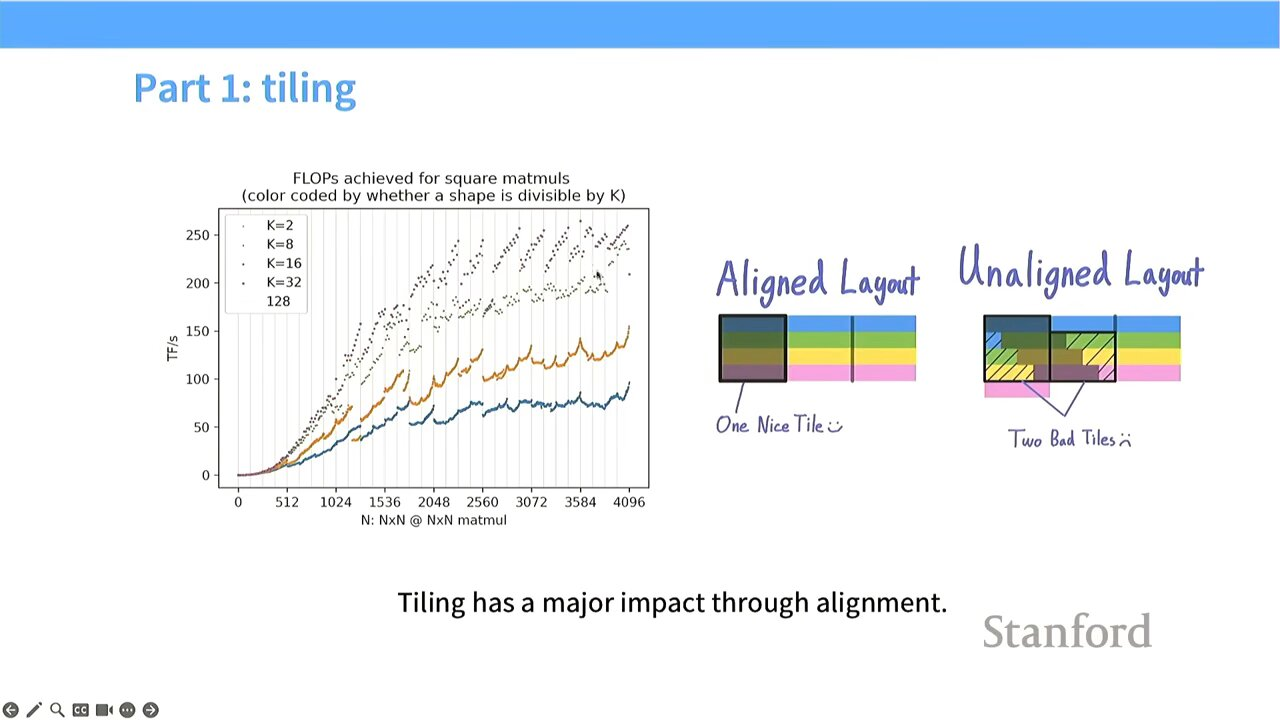
\includegraphics[width=\textwidth]{figures/fig_24_matmul_mystery_explained.jpg}
\caption{矩阵乘之谜的完整解释：内存区、分块、波量化共同作用\protect\footnotemark}
\end{figure}
\footnotetext{视频画面时间区间：00:59:45--01:00:00。}

\begin{itemize}
\item \textbf{最左段（小尺寸，约 1536 以下）的塌陷}：算术强度太低，纯粹是\textbf{内存受限}。矩阵太小，光是把数据搬进来做最基本的 IO 就占满了时间，算力单元大量空转。这正是 roofline 斜线段的体现。
\item \textbf{右侧上沿（理论上限）}：尺寸足够大时，可以饱和计算单元，逼近峰值 FLOPS。这是 roofline 的水平段。
\item \textbf{中间的锯齿/塌陷}：每一处塌陷都对应一个\textbf{分块对齐}或\textbf{波量化}的边界。当矩阵尺寸恰好让 tile 数跨过整数波边界，或让 tile 起始位置错开突发段，吞吐就会突然掉下去。
\end{itemize}

\begin{figure}[H]
\centering
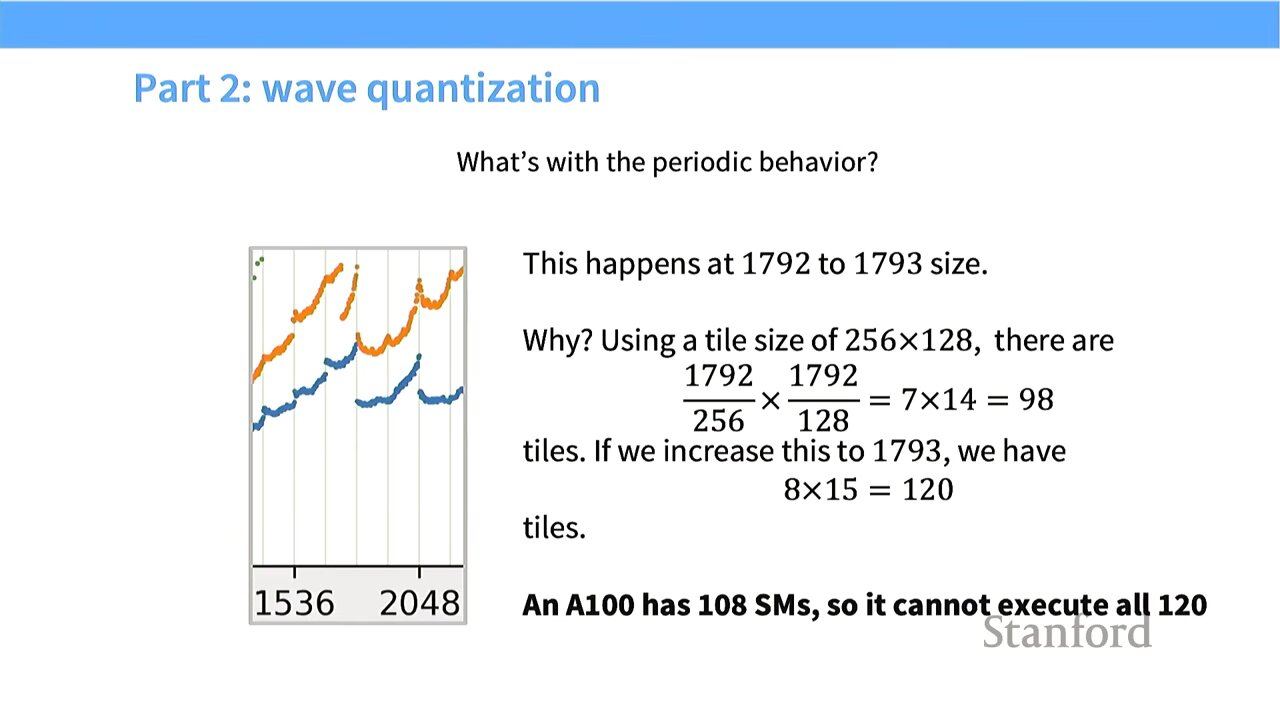
\includegraphics[width=\textwidth]{figures/fig_25_wave_quant_1792.jpg}
\caption{波量化的更宏观体现：1792 等关键尺寸处的锯齿\protect\footnotemark}
\end{figure}
\footnotetext{视频画面时间区间：01:01:15--01:01:30。}

讲师进一步指出，随着尺寸变大，波量化的"台阶"会出现在更大的尺度上（比如 1792 这种和 SM 总数、tile 大小相关的关键值）。每一段平台-塌陷-平台的锯齿，背后都是同一个机制：\textbf{工作量没能整除硬件的并行粒度}。

\subsection{Karpathy 的 vocab 优化：padding 的实战威力}

讲师引用了 Andrej Karpathy 的一条推文，展示 padding 在实战中能带来多么戏剧性的提升。\textbf{nanoGPT 最显著的单一优化，是把词表大小从 50257 改成 50304}——后者是 64 的倍数。仅仅是给词表多补了 47 个"用不到"的维度，就换来了约 \textbf{25\% 的加速}。

\begin{knowledgebox}{为什么补 47 个维度能快 25\%}
因为 50257 不能被 64（或更底层的突发段/tile 粒度）整除，导致最后一波 tile 几乎全空、SM 大量闲置，同时嵌入查表的内存访问无法合并。补到 50304 后，所有访问都对齐到突发段边界，波量化消失，吞吐直接拉满。这是"对齐就是性能"的最生动注脚。
\end{knowledgebox}

\begin{practicebox}{工程教训：永远留意你的尺寸}
在写 CUDA kernel 或调 PyTorch 时，要本能地问：\textbf{我的张量维度是不是某个常见粒度（32、64、128）的倍数？}如果不是，先 padding 到最近的倍数，往往比任何花哨的算法优化都更立竿见影。batch size、序列长度、hidden size、词表大小，都适用这条经验。
\end{practicebox}

至此，矩阵乘之谜被完全拆解：\textbf{内存瓶颈解释了左侧塌陷，分块解释了整体可达的上限，波量化与突发段对齐解释了所有锯齿}。GPU 的性能不再是黑箱，而是一组可预测、可调优的规律。

\section{实战：Flash Attention}

最后，讲师把前面所有技巧综合起来，完整地走一遍 \textbf{Flash Attention}——这篇 2022 年的论文是 GPU 优化思维的集大成者，它把 attention 的 HBM 访问从二次降到了亚平方。

\subsection{问题：标准 Attention 的 HBM 访问是二次的}

回顾标准 attention。给定 query $Q$、key $K$、value $V$（都是 $N \times d$），attention 的计算是：

\[
S = Q K^{\top}, \qquad P = \text{softmax}(S), \qquad O = P V
\]

朴素实现把它拆成三个独立的 kernel：算 $S$（写回 HBM）、算 $P = \text{softmax}(S)$（读 $S$、写 $P$）、算 $O = P V$（读 $P$）。中间矩阵 $S$ 和 $P$ 都是 $N \times N$，要被完整地写进再读出 HBM。于是\textbf{HBM 访问量是 $O(N^2)$}，随序列长度二次增长——这正是长序列 attention 又慢又占显存的根源。

\begin{figure}[H]
\centering
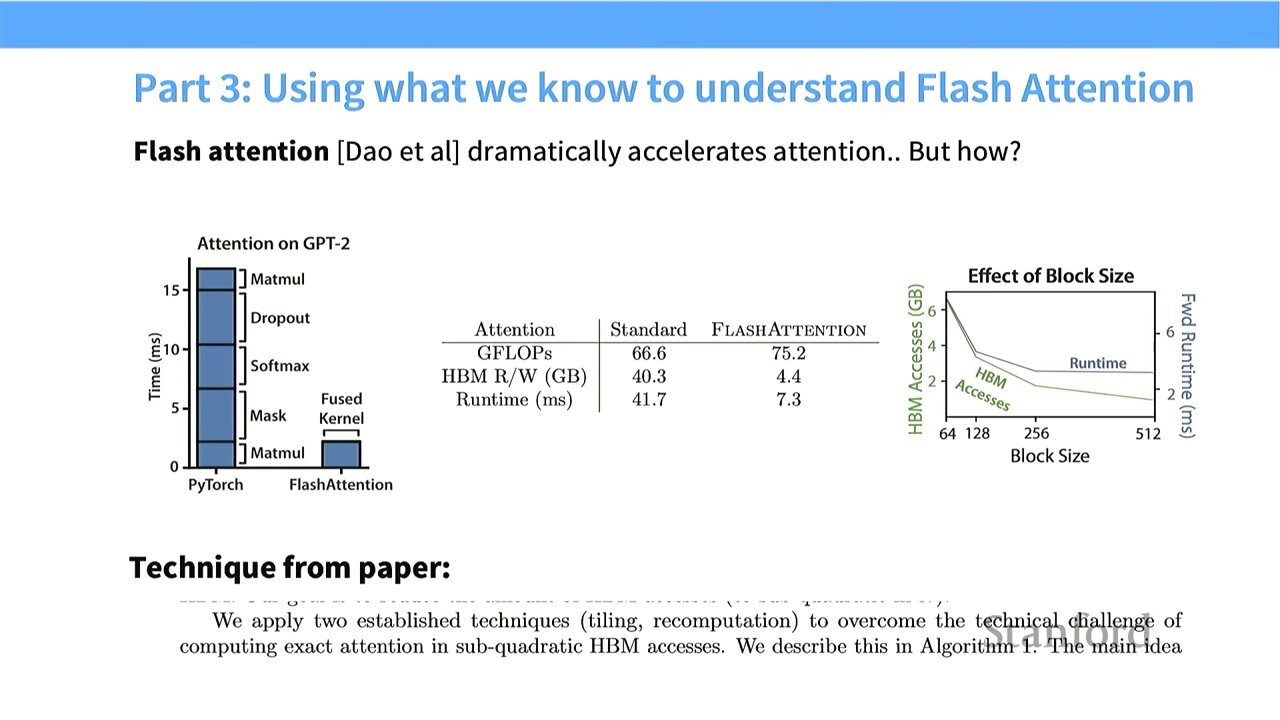
\includegraphics[width=\textwidth]{figures/fig_26_flash_attention_intro.jpg}
\caption{Flash Attention 目标：让 attention 对 HBM 的访问降到亚平方\protect\footnotemark}
\end{figure}
\footnotetext{视频画面时间区间：01:04:45--01:05:00。}

Flash Attention 的目标是：\textbf{不把 $N \times N$ 的 $S, P$ 完整物化到 HBM}。要做到这点，需要两个关键思想——\textbf{分块}（把 $Q, K, V$ 切成块，在共享内存里算）和\textbf{重计算}（不存中间的 $S, P$，需要时在共享内存里重算）。

朴素 attention 的 HBM 访问量约为：

\[
\text{HBM IO}_{\text{naive}} = O(N^2 + N \cdot d)
\]

其中 $O(N^2)$ 来自读写完整的 $S, P$ 矩阵。当 $N \gg d$ 时，$O(N^2)$ 主导。

\begin{figure}[H]
\centering
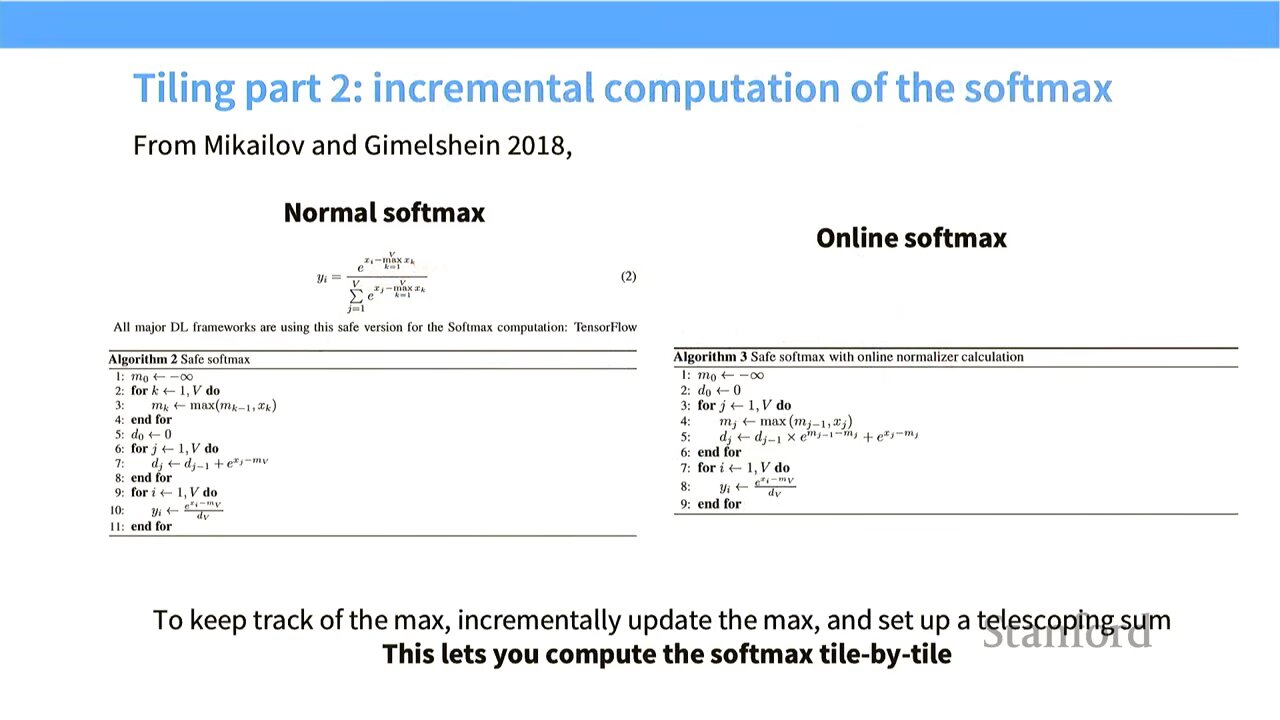
\includegraphics[width=\textwidth]{figures/fig_27_flash_attention_hbm.jpg}
\caption{Flash Attention 的 HBM 读写分析：只读写 Q,K,V,O，不物化 S,P\protect\footnotemark}
\end{figure}
\footnotetext{视频画面时间区间：01:07:30--01:07:45。}

整体流程是：把 $Q, K, V$ 切成块，每次只把一小块 $Q$、一小块 $K$、一小块 $V$ 从 HBM 搬进共享内存，在共享内存里算出这部分 attention 的贡献，累加到输出 $O$，然后\textbf{只把最终 $O$ 写回 HBM}。中间的 $S, P$ 全程只在共享内存里存在，绝不落盘。设共享内存大小为 $M$、head 维度为 $d$，分块后每块大小约为 $M/d$，则 HBM 访问降为：

\[
\text{HBM IO}_{\text{flash}} = O\!\left(\frac{N^2 d^2}{M}\right)
\]

由于 $M$ 是常数，在 $N$ 很大时这远小于 $O(N^2)$，对序列长度呈亚平方增长。

\subsection{关键障碍：softmax 不是"在线"的}

分块听起来美好，但有一个拦路虎：\textbf{softmax 里有全局归一化}。完整的 softmax 是：

\[
\text{softmax}(s)_i = \frac{e^{s_i}}{\sum_j e^{s_j}} = \frac{e^{s_i - m}}{\sum_j e^{s_j - m}}, \qquad m = \max_j s_j
\]

注意分母 $\sum_j e^{s_j}$ 和分子里的 max，都需要\textbf{看到整行}（所有 $j$）才能算。如果分块逐块算，每块只能看到部分列的 $K$，怎么能在还没看到所有列的情况下算出正确的 softmax 分母和 max？

\begin{figure}[H]
\centering
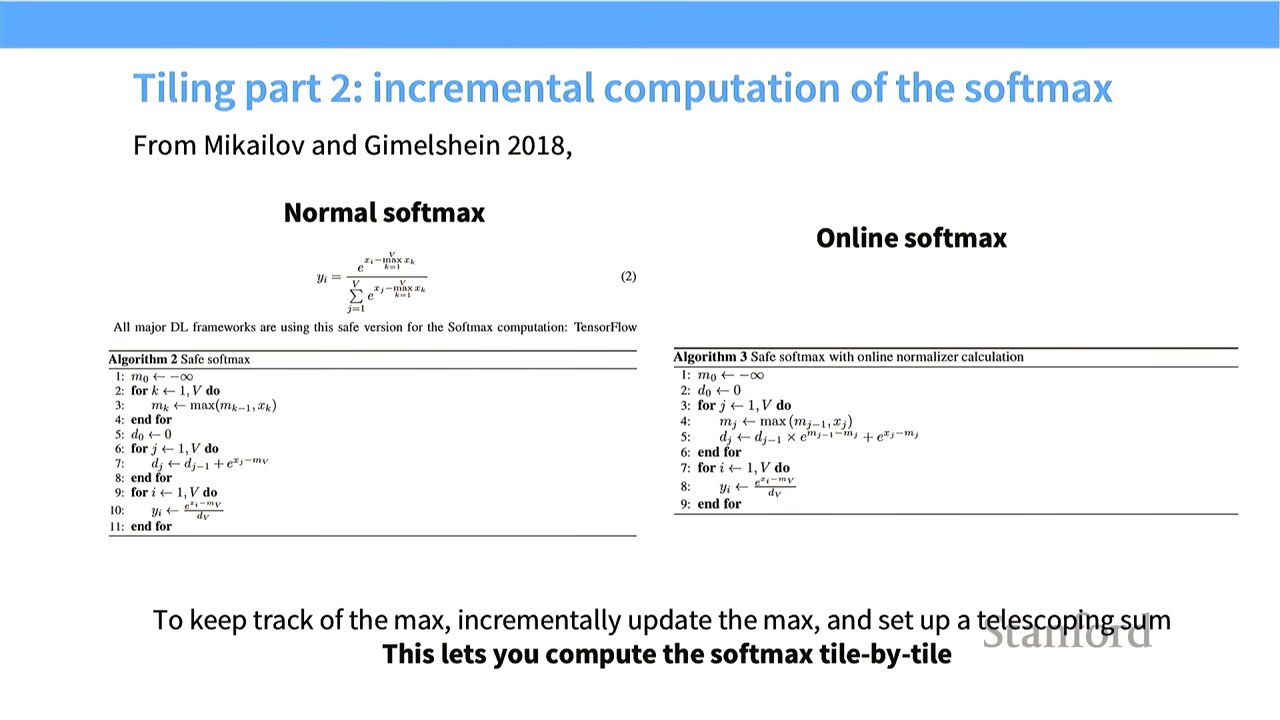
\includegraphics[width=\textwidth]{figures/fig_28_online_softmax.jpg}
\caption{Online softmax：流式更新 running max 与归一化项\protect\footnotemark}
\end{figure}
\footnotetext{视频画面时间区间：01:08:15--01:08:30。}

这就是 \textbf{online softmax} 技巧登场的地方。它的核心是维护一个\textbf{运行的最大值} $m$ 和一个\textbf{运行的指数和} $\ell$，并在每处理一个新块时，用\textbf{校正项}把之前的累加结果修正到新的 max 下。设当前已处理得到 $(m_{\text{old}}, \ell_{\text{old}})$，新来一块算出局部 $(m_{\text{new}}, \ell_{\text{block}})$，则更新规则为：

\[
m_{\text{new}} = \max(m_{\text{old}}, m_{\text{block}})
\]

\[
\ell_{\text{new}} = e^{m_{\text{old}} - m_{\text{new}}} \cdot \ell_{\text{old}} \;+\; e^{m_{\text{block}} - m_{\text{new}}} \cdot \ell_{\text{block}}
\]

这里 $e^{m_{\text{old}} - m_{\text{new}}}$ 就是那个\textbf{校正项}：当 max 被更新后，之前累加的指数和必须按新旧 max 的差重新缩放，才能和新增块在同一尺度下相加。对输出 $O$ 也做同样的缩放校正：

\[
O_{\text{new}} = \frac{1}{\ell_{\text{new}}} \Big( e^{m_{\text{old}} - m_{\text{new}}} \cdot \ell_{\text{old}} \cdot O_{\text{old}} \;+\; e^{m_{\text{block}} - m_{\text{new}}} \cdot \ell_{\text{block}} \cdot O_{\text{block}} \Big)
\]

\begin{knowledgebox}{online softmax 的精妙}
online softmax 让 softmax 从"需要一次性看到全部数据"变成了"可以逐块流式处理"，而结果在数学上与标准 softmax \textbf{严格等价}（只是浮点误差差异）。这是算法层面的巧思——它把一个看似必须全局的运算，改造成了局部的、可分块的运算，从而让 attention 的分块化成为可能。
\end{knowledgebox}

\subsection{把技巧串起来：Flash Attention 的全貌}

现在可以把所有拼图拼上了。Flash Attention 同时用到了本讲讲的几乎全部技巧：

\begin{importantbox}{Flash Attention 用到的技巧清单}
\begin{itemize}
\item \textbf{分块（tiling）}：把 $Q, K, V$ 切块，在共享内存里算，避免物化 $N \times N$ 矩阵。
\item \textbf{重计算（recomputation）}：不存中间 $S, P$，反向时重新算（用保存的 $O, m, \ell$ 做锚点）。
\item \textbf{算子融合（fusion）}：把 $S=QK^\top$、$P=\text{softmax}(S)$、$O=PV$ 融合成单个 kernel，中间结果不落 HBM。
\item \textbf{内存合并（coalescing）}：块大小设计为对齐突发段，保证搬运高效。
\item \textbf{低精度}：实际实现中 $Q,K,V$ 用 FP16/BF16，累加在 FP32。
\end{itemize}
\end{importantbox}

Flash Attention 2 进一步优化了\textbf{warp 间的工作划分}——把 $Q$ 块分配到不同的 warp 并行计算，减少 warp 间的同步与通信开销。这是"对硬件执行模型（warp、SM）的精雕细琢"如何带来巨大收益的又一例证。

\begin{practicebox}{Flash Attention 的实战意义}
\begin{itemize}
\item \textbf{训练加速}：HBM 访问大减，长序列 attention 不再是显存与带宽黑洞。
\item \textbf{显存节省}：不物化 $N \times N$ 的 attention 矩阵，显存从 $O(N^2)$ 降到 $O(N)$，让训练超长上下文成为可能。
\item \textbf{即插即用}：数学上与标准 attention 等价，不需要改模型结构，今天已是所有主流框架（PyTorch SDPA、FlashAttention 库）的默认实现。
\end{itemize}
\end{practicebox}

\section{总结与延伸}

\subsection{本讲核心要点回顾}

回顾整讲，我们从一个朴素的愿望——"让 GPU 不再神秘"——出发，层层深入：

\begin{enumerate}
\item \textbf{设计哲学}：CPU 优化延迟，GPU 优化吞吐；Dennard 缩放终结后，并行缩放成为算力增长的主引擎。
\item \textbf{硬件结构}：GPU = 大量 SM（每 SM 内含 SP + 张量核）+ 分层内存（寄存器 / 共享 / L2 / 全局 HBM）。A100 有 128 个 SM。
\item \textbf{执行模型}：CUDA 程序以 grid $\to$ block $\to$ warp（32 线程）$\to$ thread 层次执行，SIMT 让同 warp 线程锁步执行同一指令。
\item \textbf{性能分析}：roofline 模型用算术强度判定内存/计算瓶颈；矩阵乘之谜的全部特征（左侧塌陷、右侧上限、中间锯齿）都能用内存瓶颈、分块、波量化解释。
\item \textbf{五大技巧}：低精度、算子融合、重计算、内存合并、分块。它们共同的思想是\textbf{用充裕的算力换稀缺的带宽/显存}。
\item \textbf{综合实战}：Flash Attention 把上述技巧全部用上，让 attention 对 HBM 的访问降到亚平方，并给出 online softmax 这一关键算法创新。
\end{enumerate}

\subsection{一个统一的思维框架}

\begin{knowledgebox}{用 roofline 贯穿全局}
本讲所有内容都可以挂在一个框架下：\textbf{你的负载落在 roofline 的哪一段？}
\begin{itemize}
\item 落在斜线段（内存受限）$\to$ 用低精度（减字节数）、算子融合（减少往返）、分块（搬到共享内存）、内存合并（提高有效带宽）。
\item 落在水平段（计算受限）$\to$ 用低精度（张量核提速）、减少冗余计算。
\item 尺寸不对齐 $\to$ padding、调整 tile size，避免波量化与突发段错位。
\end{itemize}
每次遇到 GPU 性能问题，先用 roofline 定位，再对症下药。这是从本讲能带走的最有价值的"心智模型"。
\end{knowledgebox}

\begin{warningbox}{不可忽视的工程现实}
GPU 性能优化是一个\textbf{多层次、多约束}的耦合问题：tile size 既要够大以减少全局访存，又不能超过共享内存；既要对齐突发段，又要整除矩阵维度；既要合并访问，又要避免 warp 分叉。这些约束相互牵扯，没有万能公式。\textbf{工具（torch.compile、Triton、cuDNN）已经把大多数常见模式优化得很好}，理解原理的意义，在于知道什么时候该信任工具、什么时候得自己下手。
\end{warningbox}

\subsection{延伸阅读与下一步}

讲师在课上反复推荐的资源包括：Hennessy 与 Patterson 的《计算机体系结构：量化方法》（尤其是关于 Dennard 缩放与并行革命的章节）、Google 的 TPU 文档与配套书籍、以及 NVIDIA 的 CUDA C++ Programming Guide（关于 SM、warp、内存层次的权威说明）。在算法层面，强烈建议精读 Flash Attention 原论文（Dao 等人，2022）及其第二版，对照本讲的内容去理解每一处设计选择背后的硬件动机。

下一讲将进入\textbf{并行与分布式训练}的主题，讨论如何把多个 GPU/TPU 通过互联（NVLink、InfiniBand）连起来，以及数据并行、张量并行、流水线并行等策略。届时会发现，本讲学到的"算力 vs 带宽""分块""通信与计算重叠"等思想，在更大规模的系统上同样适用，只是瓶颈从单卡内存变成了跨设备的网络。

\begin{practicebox}{动手练习建议}
\begin{enumerate}
\item 用 \texttt{torch.utils.benchmark} 测一段矩阵乘，画出实测 TFLOPS vs 矩阵尺寸的曲线，亲手找到波量化塌陷点。
\item 把词表/hidden size 从非对齐改成 64/128 的倍数，对比吞吐变化，复现 Karpathy 的 nanoGPT 现象。
\item 读 Flash Attention 的 CUDA/Triton 实现，找出 tiling、online softmax、warp 划分对应的代码段。
\item 用 \texttt{torch.compile} 编译一个含多个逐元素算子的小网络，对比编译前后的 kernel 数量与运行时间，直观感受算子融合。
\end{enumerate}
\end{practicebox}

理解了 GPU，就理解了这个时代算力的物理底座。希望本讲之后，再看到 CUDA 报错或性能曲线时，你能少一分神秘、多一分"我知道这是怎么回事"的从容。

\end{document}
